\documentclass[journal]{IEEEtran}
\usepackage{etoolbox}
\makeatletter
\patchcmd{\@makecaption}
{\scshape}
{}
{}
{}
\makeatletter
\patchcmd{\@makecaption}
{\\}
{.\ }
{}
{}
\makeatother
\def\tablename{Table}
\renewcommand{\thetable}{\arabic{table}}

\usepackage[T1]{fontenc}
\usepackage[utf8]{inputenc}
\renewcommand\thesection{\arabic{section}}
\renewcommand\thesubsection{\thesection.\arabic{subsection}}
\renewcommand\thesubsubsection{\thesubsection.\arabic{subsubsection}}

\renewcommand\thesectiondis{\arabic{section}}
\renewcommand\thesubsectiondis{\thesectiondis.\arabic{subsection}}
\renewcommand\thesubsubsectiondis{\thesubsectiondis.\arabic{subsubsection}}
\newcommand{\ue}[1]{%
\begin{tikzpicture}[#1]%
    \draw[fill = black] (.25ex,.25ex) circle (.3ex);
    \draw[thick] (.55ex,.25ex) -- (1.55ex,.25ex);%
    \draw[fill = black] (1.85ex, .25ex) circle (.3ex);
    %
\end{tikzpicture}%
}
\usepackage{amsfonts}

\usepackage{bm}
\usepackage{wrapfig}
\usepackage{multicol}
\usepackage{sepfootnotes}
\usepackage[bottom]{footmisc}
\newfootnotes{a}
%! Suppress = GatherEquations
% introduction
\anotecontent{vbsuper}{We will often use the verb form ``to super resolve'' in order to denote the use of one or more such methods.}
\anotecontent{rayleighscriterion}{The amplitude of the diffraction pattern (known as the Airy pattern) of a monochromatic point source through a circular aperture is given by \[I(\theta)\coloneqq I_{0}\left[{\frac {2J_{1}(ka\sin \theta )}{ka\sin \theta }}\right]^{2}\] where \(I_0\) is peak intensity (at the center), \(k=\frac{2\pi}{\lambda}\) is the wavenumber of the light, \(\theta\) is the angle of observation, and \(J_1\) is the Bessel function of the first kind of order one \cite{goodman2005introduction}.
	%
	It is maxima/minima of this function that Rayleigh's criterion concerns.}
\anotecontent{shotnoise}{The number of photons incident on a sensor element is distributed according to a Poisson distribution (arrivals are independent and their rate is constant). For a small number of photons the variance in total arrivals (i.e., image brightness) is high.}
\anotecontent{satelliteoptics}{Rayleigh's criterion implies that the angular resolution \(R\) of a telescope with optical diameter \(D = 2.4\text{m}\) observing visible light (\({\sim}500\text{nm}\)) is approximately \cite{doi:10.1080.14786447908639684} \[R  \approx 1.220\frac{\lambda}{D} = 1.220 \frac{500\text{nm}}{2.4\text{m}} \approx 0.06\text{arcsec}\] From an altitude of 250 km this corresponds to a ground sample distance of 6cm.
	%
	This loss of resolving power is further exacerbated by refraction through turbulent atmosphere \cite{Fried:66}.}
\anotecontent{subpixel}{For example when a point source wholly captured by one sensor element shifts to distributing energy equally amongst that same element and a direct adjacent.}

% background
\anotecontent{lexico}{Consider an \(N\) row \(\times\) \(M\) column image \(X(n, m)\).
	%
	The column-major vectorization \(bm{x}\) of the image is the \(NM\) length vector defined as \(\bm{x}(Mm + n) = X(n, m)\).}
\anotecontent{patch}{\(m \times m\) pixel window, e.g. \(3 \times 3\).}
\anotecontent{tensor}{A multidimensional array. Not to be confused with the algebraic object.}
%\anotecontent{deep-depletion}{The depletion layer is the region at the Si-SiO\(_2\) interface that is characterized by few charge carriers (electrons and holes) that occurs when a gate voltage higher than the flat-band voltage is applied. Deep-depletion is characterized by a depletion region width that is greater than that at equilibrium \cite{semiconductorbook}.}
%\anotecontent{inversion}{The term inversion means that the surface is inverted from P type to N type, or electron rich. This process is a slow thermal equilibration \cite{ccdarkcurrent}, is called dark current and at various temperatures/exposure times is a source of noise.}
\anotecontent{nyquist}{Twice the frequency of the lowest frequency component in the image. Sampling at a rate below this leads to aliasing of high frequency components as low frequency components.}
\anotecontent{depletion}{By applying a positive voltage to the gate holes are repelled and migrate through the body to ground.
	%
	This leaves a depleted region near the Si-SiO\(_2\) interface that acts as an insulator.}
\anotecontent{buriedchannel}{Buried channel as distinct from surface channel.
	%
	In surface channel the signal charge is stored at the Si-SiO\(_2\) interface, which can lead to charge trapping during the charge transfer process \cite{Bass:2009:HOT:1594759}.}
\anotecontent{ntype}{Semiconductors are classified as either \textit{n-type} or \textit{p-type}, the former being doped with negative charge carriers and the latter being doped with positive charge carriers (holes).}
\anotecontent{ccd}{CCD arrays, for example, employ \(2\times 2\) or \(3\times 3\) pixel binning, which is the practice of collapsing windows of pixels down to one pixel.}
\anotecontent{pnjunction}{The interface between a p-type semiconductor and a n-type semiconductor.}
\anotecontent{reversebias}{With the p-type material at a lower voltage than the n-type.
	%
	This causes both the holes and the electrons to flow away from the junction creating a depletion zone.}
\anotecontent{bolometer}{Late 19th century: from Greek bolē `ray of light' + -meter.}
\anotecontent{mems}{Micro-electro-mechanical systems.}
\anotecontent{fabryperot}{An optical cavity made from two parallel reflecting surfaces that passes light only when it is in resonance with the cavity.}
\anotecontent{thermistor}{An element with an electrical resistance that is a function of its temperature.}
\anotecontent{innerphotoelectric}{The photoelectric effect is the emission of electrons when light hits a material.
	%
	The inner photoelectric effect is that phenomenon in the bulk matter of semiconductors.}
\anotecontent{otf}{The optical transfer function is the spatial Fourier transform of the point spread function (the impulse response) of the optics.
	%
	Spatial here means periodic in space rather than in time.}
\anotecontent{coma}{Off-axis point sources appearing to have a tail (coma), due to variation in magnification in the image of the aperture stop.}
\anotecontent{dispersion}{A well known example of this phenomenon is the cover of Pink Floyd's classic album The Dark Side of the Moon.}
\anotecontent{fnumber}{The ratio of the system's focal length to the diameter of the aperture.}
\anotecontent{registration}{The process of aligning two or more images of the scene on a common pixel grid.}
%registration
\anotecontent{scalepyramid}{No pun intended.}
\anotecontent{threshold}{Set everything below a threshold to zero.}
\anotecontent{nms}{Pick the maximum in a neighborhood and set all other values to zero.}
\anotecontent{log}{The Laplacian of an image \(X\) is \(L(x,y) = \partial_x^2 X + \partial_y^2 X\).
	%
	Since in practice this approximates a noisy signal (second derivative), smoothing by a Gaussian is a necessary prerequisite.
	%
	Therefore the Laplacian of Gaussians (\(LoG\)) filter is the Laplacian composed with the Gaussian: \begin{equation*} LoG(x,y, \sigma) \coloneqq -\frac{1}{\pi \sigma^4}\left[ 1 - \frac{x^2+y^2}{2\sigma^2} \exp \left\{ - \frac{x^2+y^2}{2\sigma^2} \right\} \right]
	\end{equation*}}
\anotecontent{smallcurvature}{The ratio of the eigenvalues of the spatial Hessian of \(D\) (i.e., only along dimensions \(x,y\)).
	%
	In fact a quantity not unlike eqn.~\eqref{eqn:strength} is computed in order to save having to explicitly find eigenvalues.}
\anotecontent{hog}{The histogram of gradient orientations (polar angle) in a pixel window.}
\anotecontent{kdtree}{\(k\)-d trees \cite{Bentley:1975:MBS:361002.361007}, short for \(k\)-dimensional trees, are data structures that partition space efficiently in order that searching the data structure, insertion into the data structure, and deletion from the data structure are all, on average, \(O(\log n)\) time operations (where \(n\) is the number of nodes in the tree at the time of the operation).}
\anotecontent{ransac}{Random Sample Consensus (RANSAC) is a method used to estimate parameters of a model given outliers.
	%
	In this case Zahra \etal use RANSAC at the transform estimation step to eliminate falsely matched keypoint pairs.
	%
	RANSAC iterates by repeatedly random sampling the putative matching keypoint pairs and fitting a transform model.
	%
	At a given iteration the fitted transform model is tested against the heldout keypoint pairs and evaluated (according to goodness of fit on a subset called the \textit{consensus set}).}
\anotecontent{gridsearch}{Searching a space by taking regular incremental steps along each dimension. For example, search \(U \subset \mathbb{R}^2\) by checking all \(x = \Delta x + x_0, y = \Delta y + y_0\) for \((x_0, y_0) \in U\) and for fixed \(\Delta x, \Delta y\).}
\anotecontent{fouriershift}{If \(\mathcal{F}\{\left[ x_n \right] \}_{k}=X_{k}\) is the \(k\)-th frequency component of the discrete signal
\(\left[ x_n \right]\) then shifting \(\left[ x_n \right]\) by \(m\) steps implies
\[
	\mathcal{F}\left\{\left[ x_{n-m} \right]\right\}_{k} = X_{k}\cdot e^{-{\frac {i2\pi }{N}}km}
\]
}
\anotecontent{hadamard}{
	\[
		\begin{bmatrix}
			a_{11} & a_{12} \\
			a_{21} & a_{22} \\
		\end{bmatrix}\odot \begin{bmatrix}
			b_{11} & b_{12} \\
			b_{21} & b_{22} \\
		\end{bmatrix} \coloneqq
		\begin{bmatrix}
			a_{11}\,b_{11} & a_{12}\,b_{12} \\
			a_{21}\,b_{21} & a_{22}\,b_{22} \\
		\end{bmatrix}
	\]
}
\anotecontent{shannon}{
	Shannon entropy can be interpreted as the average number of bits \(L\) necessary to encode a random variable \(X\) distributed according to distribution \(P\).
	%
	It is defined as
	\[
		H(X)\coloneqq\sum{P(x)\log\left[\frac{1}{P (x)}\right]}
	\]
	i.e., \(P(x_i) = 1/2^L\) where \(L\) is the number of bits.
}
\anotecontent{kde}{Alternatively known as Parzen windowing, the kernel density estimator \(\hat{P}\) of a distribution \(X\sim P\) given a set of points \(\left\{ x_1, x_2, \dots, x_n \right\}\) is defined as
	\[
		\hat{P}(x) \coloneqq {\frac {1}{nh}}\sum _{i=1}^{n}K\left( \frac {x-x_{i}}{h} \right)
	\]
	where \(K\) is a kernel (e.g. Gaussian) and \(h\) is the \textit{kernel bandwidth}.
}
\anotecontent{convexhull}{A convex combination of points \(x_1, x_2, \dots, x_n\) is all \(\alpha _{1}x_{1}+\alpha _{2}x_{2}+\cdots +\alpha _{n}x_{n}\) where \( \alpha _{i}\geq 0\) and \(\alpha _{1}+\alpha _{2}+\cdots +\alpha _{n}=1\).
%
The convex hull of a set of points \(X\) is the set of all convex combinations of points in \(X\).
%
Figuratively one can imagine stretching a rubber band such that it contains all points in \(X\).}
\anotecontent{completegraph}{A graph in which each pair of vertices is connected by an edge.}
\anotecontent{homogeneous}{
	With \((x,y)\) a pixel coordinate, transformations \(T\) in homogeneous coordinates operate on \((x,y,1)\): if
	\(
	(a,b,c) = (x,y,1)\cdot T
	\)
	then the transformed pixel coordinate
	\(
	(x',y') = \frac{1}{c} (a,b)
	\).
}
\anotecontent{advection}{Advection is the transport of a substance, or properties thereof, by bulk flow of a fluid. The substance, or properties thereof, are \textit{advected} by the flow and are considered \textit{conserved}. In general, the fluid flow is described by a vector field \(\mathbf{u}\) (called velocity) and the substance or property is described by a scalar field \(\psi\) (variously called distribution, concentration, or density). The canonical example is the advection of ink by flowing water.}
\anotecontent{stokes}{
	The integral of a differential form \(\omega\) on the boundary of some orientable manifold \(\Omega\)  is equal to the integral of its exterior derivative \(\dif \omega\) on \(\Omega\), i.e
	\[
		\oint\limits _{\partial \Omega }\omega =\int\limits _{\Omega }\dif\omega
	\]
	In this instance \(\Omega = R\), \(\omega = \mathbf{j} \cdot \mathbf{n}\, \dif l \) and \( \dif \omega = \nabla \cdot \mathbf{j}\, \dif R\).
}
\anotecontent{tvloss}{ Total variation is equivalent to the integral of the gradient magnitude:
\[
	\abs{u}_{\operatorname {TV}}=\int\limits\abs{\nabla u}
\]
}
\anotecontent{indicator}{The indicator (or characteristic) \(\mathbbm{1}_{[a,b)}\) function is 1 on the interval \([a,b)\) and 0 otherwise.}
\anotecontent{vectorspace}{A set whose members (\textit{vectors}) can be decomposed as linear combinations of elementary elements (a \textit{basis}).}
\anotecontent{splinecontconstr}{Note that even though a \(d\)-degree polynomial has \(d\) derivatives we only require agreement at the first \(d-1\) derivatives (and continuity itself). This is owing to the fact that if we required all \(d\) derivatives to agree the number of degrees of freedom would be \((n(d+1) - (n-1)(d+1) = d+1\) and therefore the spline would no longer be a piecewise polynomial but simply a polynomial (of degree \(d\)).}



%classical
\anotecontent{delauney}{The Delaunay triangulation for a set of points \(P\) is a triangulation such that no point in \(P\) is inside the circumcircle of any triangle in the triangulation. Equivalently it is the triangulation that maximizes the minimum angle of all of the triangles in the triangulation.}
\anotecontent{estiminterp}{This blurring of the distinction between interpolation and estimation is to be expected since estimation is a type of regression.}
\anotecontent{gp}{A Gaussian process is a sequence of random variables such that any finite subset is distributed multivariate Normal.}
\anotecontent{lsi}{In analogy with Linear Time Invariant (i.e., linear and constant in space).}
\anotecontent{lrpixel}{An LR pixel is one sampled from an LR image and embedded in the HR grid.
	%
	An HR pixel is a pixel in the HR grid.}
\anotecontent{vectorize}{
	\begin{multline*}
		\text{vec}\left(
		\begin{bmatrix}
				a_{11} & a_{12} & \cdots & a_{1n} \\
				a_{21} & a_{22} & \cdots & a_{2n} \\
				\vdots & \vdots & \ddots & \vdots \\
				a_{m1} & a_{m2} & \cdots & a_{mn}
			\end{bmatrix}
		\right) = \\
		\left[a_{11}, \mathellipsis, a_{m1}, a_{12}, \mathellipsis, a_{m2}, \mathellipsis, a_{1n} \mathellipsis a_{mn}\right]
	\end{multline*}
}
\anotecontent{noise}{Noise here doesn't necessarily mean unwanted high frequency variation but simply a source of randomness.
	%
	This is in close affinity with how generative machines such as variational auto-encoders and generative adversarial networks are understood.}
%
\anotecontent{gpassumptions}{Namely \(\bm{y}_1\) is distributed \((0, W)\)-Normal and independent of \(\eta_1\).}
\anotecontent{kalmanprediction}{This is better understood in the more general linear dynamic systems case where \(\bm{y}_k = A_k\cdot\bm{y}_k + B_k \cdot \bm{u}_k + \varepsilon_k\) and \(B_k \cdot \bm{u}_k\) is known as controlled input.
	%
	Then the prediction includes a \(B_k \cdot \bm{u}_{k-1}\) term and the Kalman gain effectively mediates between controlled and uncontrolled inputs.
}
\anotecontent{hmrf}{A Markov Random Field (MRF) is a collection of random variables \(x_i, y_j, \mathellipsis\) with conditional dependence represented by pairings and satisfying the \textit{pairwise Markov} property: any two random variables that aren't paired are conditionally independent of each other given (conditioned on) all other variables.
	%
	A \textit{Hidden} Markov Random Field is simply a MRF where some of the random variables aren't observed.
}
\anotecontent{locallinear}{An LR patch \(x_i\) on the LR manifold and its neighbors \(x_j, x_k, \mathellipsis\) lie in a locally linear subspace of the manifold.}
\anotecontent{forest}{A tree is a graph in which any pair vertices is connected by exactly one or zero edges. A forest is a disjoint collection of trees.}
\anotecontent{positivedef}{A symmetric real matrix \(Q\) is positive definite if \(\bm{y}^T Q \bm{y} > 0 \) for all non-zero \(\bm{y}\).}
\anotecontent{conjugategradients}{Two vectors \(\bm{u}, \bm{v}\) are conjugate with respect to \(G\) if \(\bm{u}^T G \bm{v} = 0\).
	%
	Conjugate gradient descent is gradient descent but with conjugate gradients (it has better convergence properties).
}
\anotecontent{illcondition}{The condition number \(\kappa\) of a function is a measure of how sensitive it is to small perturbations; for a matrix \(G\) it is defined \(\kappa (G) \coloneqq \sigma_{\max}(G)/\sigma_{\min} (G)\) where \(\sigma_{\max}(G), \sigma_{\min} (G)\) are the maximum and minimum singular values of \(G\) respectively.}
\anotecontent{precondition}{A preconditioner of a matrix \(G\) is an approximation of \(G\) that has a better condition number.
	%
	Nguyen \textit{et al.} propose a preconditioner with singular values clustered around 1 in order that \(\kappa(G) \approx 1\).}
\anotecontent{gradientoperator}{Let \(u = (1,2,1)\) and \(v = (1,0,-1)\) then \(h = uv^T\) is the first order Sobel filter and \(\nabla Y = \left( h \ast Y, h^T \ast Y \right)\).}
\anotecontent{boundedvariation}{\(f(x)\) is of bounded variation on interval \(\left[ a,b \right]\) if over all partitions \(\mathcal{P}\) of \(\left[ a,b \right]\)
	\[
		\sup_{P \in \mathcal{P}}\sum_{i=0}^{n_P-1} \lvert f(x_{i+1})-f(x_i) \rvert\, <\infty
	\]
}
\anotecontent{beliefpropagation}{An efficient way to compute marginals of joint probabilities that have structure by reusing partial sums (i.e., passing messages) \cite{Yedidia2003jan1}.}
\anotecontent{manifold}{A collection of points that locally resembles Euclidean space.}
\anotecontent{manifoldlearning}{Dimensionality reduction.}
\anotecontent{pun}{No pun intended.}
\anotecontent{overcompletedictionary}{A collection of vectors (known as \textit{atoms}) that spans a space but is also linearly dependent.}
\anotecontent{nphard}{Problems in NP are those which are unknown to have a deterministic polynomial time solutions.
	%
	An NP-hard problem admits a polynomial time reduction from any problem in NP (colloquially they are as hard as any problem in NP).}
\anotecontent{firstordergaussian}{The first derivative of the Gaussian expressed as a filter: \(\left[ -2,-1,0,1,2 \right]\).}

% ann
\anotecontent{ann}{Artificial neurons are loosely inspired by the spiking neuron model of biological neurons, where dendrites correspond to inputs, the soma corresponds to a linear sum of inputs, and axons corresponds to the activation function.}
\anotecontent{bias}{The semantics of bias are inherited from from statistics, where the bias of an \textit{estimator} is the extent to which the estimator, on average, differs from the value being estimated. Therefore, if we regard an artificial neuron as an estimator (a nonlinear regression), we see that the constant term \(b\) indeed determines its bias.
}
\anotecontent{xor}{Exclusive-Or \(\operatorname{XOR}(a,b)\) is a Boolean function (maps \(\{0,1\}\) to \(\{0,1\}\)) defined to be 1 when \(a \neq b\) and 0 otherwise.}
\anotecontent{backprop}{Backprop itself is a particular instance of a general technique called automatic differentiation (AD). AD computes exact derivatives of functions in either \textit{forward accumulation} or \textit{reverse accumulation} \cite{linnainmaa1976taylor}. Backprop corresponds to reverse mode. In reverse mode the dependent variable \(y\) to be differentiated is fixed and the derivative is computed with respect to each sub-expression \(z_i\) recursively:
	\begin{multline*}
		{\frac  {\partial y}{\partial w}}={\frac  {\partial y}{\partial z_{1}}}{\frac  {\partial z_{1}}{\partial w}}=\left({\frac  {\partial y}{\partial z_{2}}}{\frac  {\partial z_{2}}{\partial z_{1}}}\right){\frac  {\partial z_{1}}{\partial w}}=\\\left(\left({\frac  {\partial y}{\partial z_{3}}}{\frac  {\partial z_{3}}{\partial z_{2}}}\right){\frac  {\partial z_{2}}{\partial z_{1}}}\right){\frac  {\partial z_{1}}{\partial w}}=\cdots 
	\end{multline*}
}
\anotecontent{universapprox}{Given enough layers and neurons ANNs with nonlinear activations are able to represent functions of arbitrary complexity. Conversely, sans a nonlinear activation function, ANNs are unable to represent functions as simple as even \(\operatorname{XOR}\).}
\anotecontent{learn}{To learn, in this context, means to approximate a function that effectively performs a task. For example in the case of an object recognition task, learning entails approximating a function that outputs high values when an object is recognized and low values otherwise.}
\anotecontent{largeparams}{OpenAI’s Generative Pre-trained Transformer (GPT) \cite{radford2018improving} natural language processing (NLP) network has approximately 150 million parameters (and takes 8 GPU-months of non-stop training).}
\anotecontent{kldiv}{The Kullback–Leibler divergence of two probability distributions \(P,Q\) with densities \(p, q\) is defined
	\begin{equation*}
		\operatorname{D}_{\text{KL}}(P\parallel Q)\coloneqq\int\limits _{-\infty }^{\infty }p(x)\log \left({\frac {p(x)}{q(x)}}\right)\,dx
	\end{equation*}
Note that \(\operatorname{D}_{\text{KL}}\) is not symmetric and therefore not a true distance measure. Fortunately it can be symmetrized:
\begin{equation*}
	\operatorname{JSD}(P\parallel Q)\coloneqq{\frac  {1}{2}}\operatorname{D}_{\text{KL}}\left(P\bigg\| {\frac  {1}{2}}(P+Q)\right)+{\frac  {1}{2}}\operatorname{D}_{\text{KL}}\left(Q\bigg\| {\frac  {1}{2}}(P+Q)\right)
\end{equation*}
In this form it is called the Jensen–Shannon divergence and is a true distance measure between probability distributions.
}
\anotecontent{minimax}{Strictly speaking mini-max is a decision rule followed by each player of a game --- a decision rule that leads to minimizing the possible loss for a worst case (maximum loss) scenario.}
\anotecontent{uniformconv}{A sequence of functions \(F_n\), \textit{uniformly converges} to \(f\) on a bounded interval \(I\) if given some \(\varepsilon > 0\) there exists \(n\) such that 
\[
	\abs{ F_n( x ) - f ( x ) } < \varepsilon
\]
for all \(x \in I\). Note the order of the quantifiers: there should be \textbf{one} \(n\) that satisfies the constraint at a given precision \(\varepsilon\) for \textbf{all} \(x \in I\) simultaneously.
}
\anotecontent{annealing}{Learning rate annealing imposes a scheduled decay of the learning rate \(\alpha_i\) over time. The intuition being that initially, prior to identifying a minimum, one can afford to take optimistically large steps \(\Delta w_i\) in parameter space but over time one should become more conservative in order to hone in on an identified minimum. Typically the annealing schedule is such that the learning rate out starts out large and is reduced by an order of magnitude (i.e., a factor of 10) every \(M\) epochs (where \(M\) is a divisor of the total number of epochs that one will train for).}
\anotecontent{gradclip}{Exploding gradients is the opposite of vanishing gradients: gradients become so large that weights become unstable. That is, weight updates become large and oscillate around a minimum. Gradient clipping constrains \(\pd{L}{w_i}\) to be within a narrow range around 0; Kim \etal constrain the gradient to be within \(\left[ -\frac{\theta}{\alpha_i}, \frac{\theta}{\alpha_i} \right]\) for some small \(\theta\).}
\anotecontent{ntire}{The performances of various techniques on SISR and MISR tasks are evaluated at a competition held at the annual New Trends in Image Restoration and Enhancement (NTIRE) workshop. The competition \cite{nah2019ntire} has two tracks: a clean track that only assumes down-sampling test cases and a blur (or natural) track that assumes motion blur (in an effort to approximate real conditions). Many teams compete in both tracks.}

% conclusions
\anotecontent{transfer}{Given a source domain and target domain, transfer learning sets out to accelerate learning for a task over the target domain using learning already performed for a task over the source domain.}
\anotecontent{tremor}{For example Physiologic tremor in the case of cell phone cameras. Physiologic tremor is a low amplitude tremor of a limb that presents at approximately 10Hz. It occurs in normal, healthy individuals.}
\anotecontent{rl}{Reinforcement Learning is a paradigm of machine learning based on principles of operant conditioning, i.e., using punishment and reward.}
\anotecontent{rnn}{A Recurrent Neural Network (RNN) models time dependencies in sequences of data.}

% appendix
\anotecontent{diracdelta}{A generalized function is a function that can only be integrated against. Let 
\begin{equation*}
	\delta_\epsilon(x) \coloneqq \frac{1}{\epsilon \sqrt{\pi}}	e^{-x^2/\epsilon^2}
\end{equation*}
Then for any continuous \(\phi(x)\)
\begin{equation*}
	\lim_{\epsilon\rightarrow 0} \left[\int\limits_{-\infty}^{\infty} \phi(x)\delta_{\epsilon}(x-x_0) \right] = \lim_{\epsilon\rightarrow 0} \left[ \phi(x_0)\int\limits_{-\infty}^{\infty} \delta_{\epsilon}(x-x_0) \right] = \phi(x_0)
\end{equation*}
and hence \(\delta(x)\) is defined as the limit of this behavior
\begin{equation*}
	\int\limits_{-\infty}^{\infty} \phi(x)\delta(x-x_0) = \phi(x_0)
\end{equation*}
}
\usepackage[pdftex]{graphicx}
\usepackage[hyperfootnotes=false]{hyperref}\usepackage{amsmath}

\usepackage[backend=biber, bibencoding=utf8, style=ieee]{biblatex}
%\usepackage[backend=bibtex, bibencoding=utf8, style=ieee]{biblatex}
\addbibresource{quals.bib}
\usepackage{tikz}
\usetikzlibrary{positioning}
\usetikzlibrary{shapes,arrows}
\usepackage[edges]{forest}
\usepackage{adjustbox}
\usepackage{mathtools}
\usepackage{breqn}
\usepackage{subcaption}

% Note that the amsmath package sets \interdisplaylinepenalty to 10000
% thus preventing page breaks from occurring within multiline equations. Use:
\interdisplaylinepenalty=0

% fix footnote rule from ieee
\def\footnoterule{\relax%
\kern-5pt
\hbox to \columnwidth{\hfill\vrule width 0.5\columnwidth height 0.4pt\hfill}
\kern4.6pt}


\begin{document}
    \title{Super Resolution for Automated Target Recognition}
    \author{Maksim Levental}
    \maketitle

    \begin{abstract}
        Super resolution is the process of producing high-resolution images from low-resolution images while preserving ground truth about the subject matter of the images and potentially inferring more such truth.
        %
        Algorithms that successfully carry out such a process are broadly useful in all circumstances where high-resolution imagery is either difficult or impossible to obtain.
        %
        In particular we look towards super resolving images collected using longwave infrared cameras since high resolution sensors for such cameras do not currently exist.
        %
        We present an exposition of motivations and concepts of super resolution in general and current techniques, with a qualitative comparison of such techniques.
        %
        Finally we suggest directions for future research.
    \end{abstract}

    \section{Introduction}\label{sec:introduction}
    \section{Introduction}\label{sec:introduction}
\noindent{\vrule width \columnwidth height 0.4pt}

Super-resolution (SR) is a collection of methods\anote{vbsuper} that augment the resolving power of an imaging system.
%
Here, and in the forthcoming, by resolving power we mean the ability of an imaging device to distinguish distinct but proximal objects in a scene.
%
If such objects are modeled as point sources of light then the resolving power of the imaging system is defined by Rayleigh's criterion: two point sources are considered \newterm{resolved} when the first diffraction maximum\anote{rayleighscriterion} of one point source coincides (at most) with the first minimum of the other (see figure~\ref{fig:rayleigh}).
\begin{figure}[!htbp]
	\center
	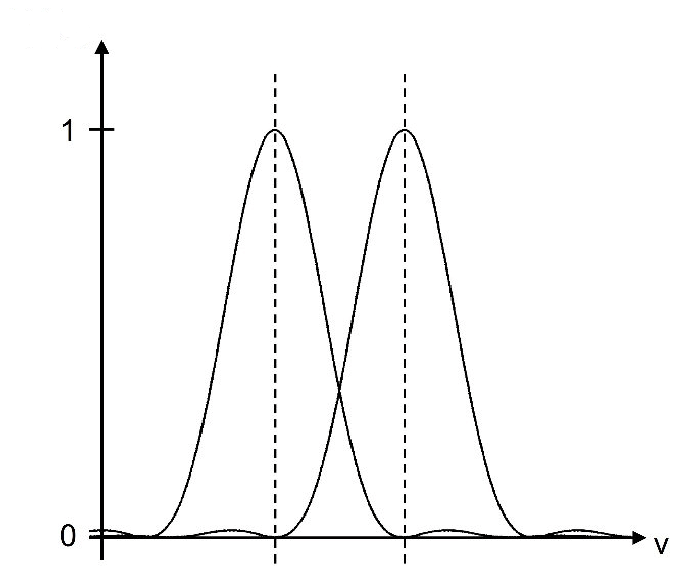
\includegraphics[width=\linewidth,keepaspectratio]{figures/classical/rayleigh.png}
	\caption{Rayleigh's criterion. Dashed lines indicate diffraction maxima and minima \cite{rayleigh}.}
	\label{fig:rayleigh}
\end{figure}

SR techniques yield high-resolution (HR) images from one or more observed low-resolution (LR) images by restoring lost fine details and reversing deterioration produced by imperfect imaging systems.
%
In the case where a single LR source image is used to construct the HR correspondent, the techniques are referred to as single-image-super-resolution (SISR) techniques.
%
These techniques typically operate either by constructing a mapping from low resolution patches\anote{patch} to higher resolution patches or by estimating the HR image given the LR image.
%
In the case when multiple LR source images are used to construct a single HR correspondent, the techniques are referred to as multiple-image-super-resolution (MISR) techniques.
%
MISR techniques rely on non-redundant and pertinent information in multiple images of the same scene (see figure~\ref{fig:misr}).
\begin{figure}[!htbp]
	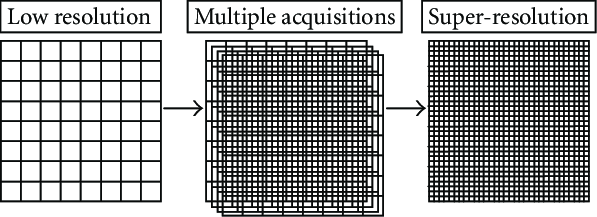
\includegraphics[width=\linewidth,keepaspectratio]{figures/classical/misr.png}
	\caption{Multiple image super resolution. Multiple low resolution images are superposed on a higher resolution grid in order to recover non-redundant information \cite{misr}.}
	\label{fig:misr}
\end{figure}
%
Note that for such information to exist there should be sub-pixel\anote{subpixel} shifts in either the imaging system or the scene between consecutive images.

For typical imaging use-cases higher resolutions are
desirable in and of themselves and as inputs to later image processing transformations that can further degrade image quality.
%
In theory the resolving power of an imaging system is primarily determined by the number of independent sensor elements that comprise that imaging system (each of which collects a component of the ultimate image).
%
Naturally then, a way to increase the resolution of such a system is to increase the density of such sensor elements per unit area.
%
Unfortunately, and counter-intuitively, since the number of photons incident on each sensor decreases as the sensor shrinks, shot noise\anote{shotnoise} thwarts that idea.
%
Furthermore, while sensor density is primary, secondary effects limit resolution as well.
%
For example, the point spread of a lens (distortion of a point source due to diffraction), chromatic aberrations (distortion due to differing indices of refraction for differing wavelengths of light), and motion blur all work to obscure or erase details from the image.


In domains such as satellite/aerial photography, medical imaging, and facial recognition,
high-resolution reconstruction of low-resolution samples is eminently useful since ab-initio acquisition of high-resolution images is either logistically difficult or impossible.
%
For example, in the case of satellite imagery, acquisition of high-resolution imagery is primarily hampered by optics and physics\anote{satelliteoptics}.
%
In contrast, in the case of medical imaging, where patient exposure time needs to be minimized \cite{doi:10.1002.cmr.a.21249}, the primary challenges are logistics and access to repeat collection opportunities.

The benefits of enhancing images using SR techniques include not only more pleasing or more readily interpretable images for human consumption, but higher quality inputs for automated learning systems as well.
%
Indeed this is our ultimate goal --- not super-resolution per se but super-resolution in the service of improved object detection performance for longwave-infrared (LWIR) imagery.
%
Towards that end, we do not consider hardware solutions for increasing the resolution of an imaging system.
%
We instead take low resolution images as given produce of a fixed imaging system and explore techniques that allow for ex post facto recovery or inference of precise details.
%
This necessarily constrains techniques under consideration to be algorithmic in nature and software in practice.

The rest of this survey is outlined as follows: section~\ref{sec:background} introduces imaging systems, notation, and the mathematical framework for the proceeding sections, section~\ref{sec:registration} surveys image registration techniques (a necessary pre-processing step for MISR), section~\ref{sec:classical-algorithms} surveys classical techniques (those that do not employ neural networks), section~\ref{sec:neural-networks} surveys neural network techniques with heavy emphasis on deep learning, and finally section~\ref{sec:conclusions} concludes with a brief discussion of future research directions.
    %
    \section{Background}\label{sec:background}
    \subsection{Imaging systems}\label{subsec:imaging-systems}
\begin{figure}
	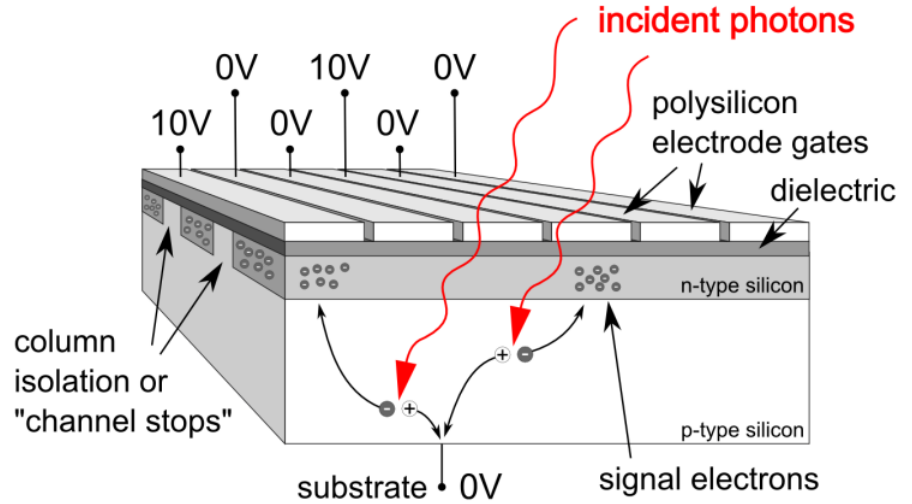
\includegraphics[width=\linewidth,keepaspectratio]{figures/background/bccd.png}
	\caption{CCD buried channel MOS capacitor\cite{finaltestguideline}}
	\label{fig:mos-cap}
\end{figure}
We begin with a practical discussion of imaging systems.
%
An imaging sensor is a device that converts an optical image into a digital signal.
%
Charge-coupled devices (CCD) and complementary metal-oxide-semiconductor (CMOS) devices are the most common imaging sensors;
%
CCDs have better performance while CMOS devices are newer and less expensive.
%
A third type that's of particular interest to us is the microbolometer, which is used as a sensor in thermal cameras.
\subsubsection{CCD Devices}
CCDs consist of densely packed two-dimensional arrays of buried channel\anote{buriedchannel} MOS capacitors (see figure~\ref{fig:mos-cap}) with an individual MOS capacitor being the fundamental photon detecting element.
%
Individual MOS capacitors are biased by a gate voltage such that a potential well is produced in the n-type silicon (referred to as the n-channel).
%
This potential well acts as a storage system for charge induced by the inner photoelectric effect\anote{innerphotoelectric}.
%
When photons are incident on a MOS capacitor some of the photons are absorbed, some are scattered, and some are transmitted.
%
Those photons that are transmitted interact with electrons in the valence band of the silicon exciting them into the conduction band, and thereby create electron-hole pairs that either diffuse or recombine.
%
For high-quality silicon, the lifetime of such a pair is several milliseconds (before recombination)\cite{scientificccd}.
%
The electrons of the electron-hole pairs that do not recombine diffuse into the potential well, while the holes migrate to the grounded substrate (i.e. out of the sensor).
%
Electrons created in this way are called \textit{photoelectrons}.

CCD arrays consist of two sub-arrays: an image section and a readout section (see figure~\ref{fig:ccd-array}).
%
The image section is arranged with every third stripe of electrode tied electrically to form three sets of equipotentials.
\begin{figure}
	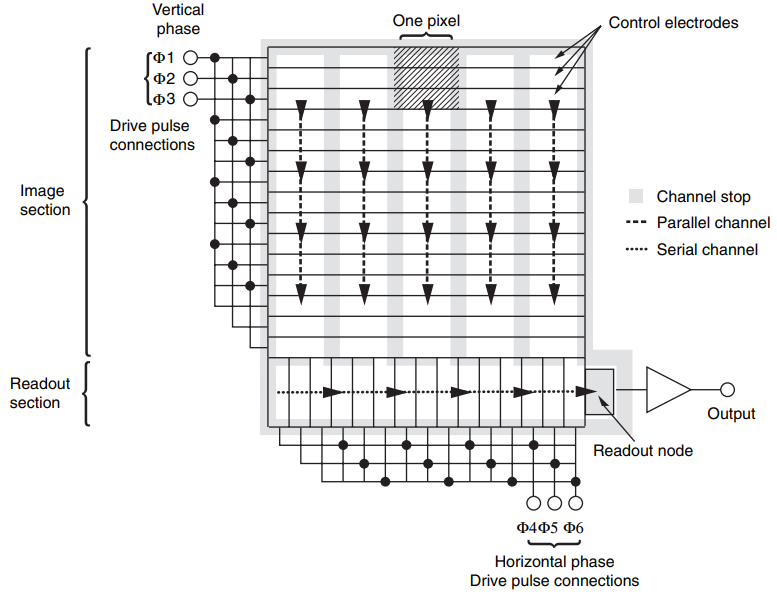
\includegraphics[width=\linewidth,keepaspectratio]{figures/background/ccd_array.png}
	\caption{CCD array\cite{pawley1995handbook}}
	\label{fig:ccd-array}
\end{figure}
%
In figure~\ref{fig:ccd-array} these equi-potentials are labeled $\Phi1, \Phi2, \Phi3$, and taken together constitute a vertical register (VR).
%
They function to move the collected photo-electrons down one electrode line at a time, using charge coupling, while the channel stops function to prevent diffusion of charge across channels.
%
The VR mechanism that shifts collected charge operates as follows:
\begin{framed}
\begin{enumerate}
	\item Suppose initially there's a collection of photo-electrons on each channel at $\Phi1$ and only $\Phi1$. Note this means $\Phi2, \Phi3$ are at $0$v (again just as in figure~\ref{fig:mos-cap}).
	\item $\Phi2$ is positively biased to $10$V. This diffuses the collection of charge under both $\Phi1$ and $\Phi2$.
	\item $\Phi1$ is set to $0$v. This concentrates the collection of charge under $\Phi2$.
	\item The same is repeated with $\Phi2, \Phi3$ and $\Phi3, \Phi1$.
	\item The entire process repeats thereby shifting the charge three lines (or one pixel row) at a time.
\end{enumerate}
\end{framed}
At the bottom of the image section $\Phi3$ transfers all signal charges to the horizontal register (HR) which functions much like the VR except faster: the HR must transfer every line of pixels independently of all other lines to the read-out node.
%
An obvious challenge faced by this system is how to prevent errant charge from accumulating out of sync with the shift process i.e. how to prevent new photoelectrons from being produced at intermediate lines while far lines are being shifted.
%
The solution is to have interstitial dedicated shift channels in between columns of sensors, with the shift channels being masked off from exposure to light.
%
This type of reading is called \textit{interline transfer} because the accumulated charge is first moved one line over, into the shift channels.
%
Naturally interline transfer shrinks photosensitive area by half and despite possible solutions (e.g micro-lenses being used to focus most of the light onto the unmasked sensors) this is one of the drawbacks of CCDs that CMOS imaging systems do not share.
\subsubsection{CMOS Devices}
CMOS sensors consist of arrays of photodiodes (see figure~\ref{fig:photodiode.png}).
\begin{figure}
	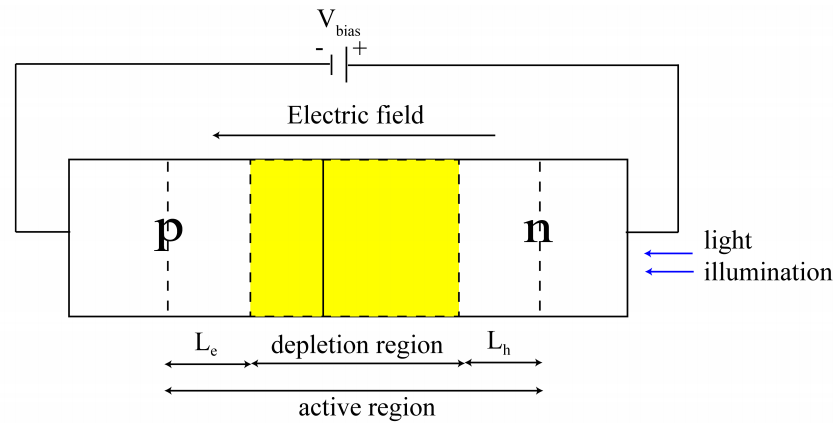
\includegraphics[width=\linewidth,keepaspectratio]{figures/background/photodiode.png}
	\caption{Photodiode schematic. L\textsubscript{e}, L\textsubscript{h} are electron, hole diffusion lengths respectively\cite{Xu2015FundamentalCO}}
	\label{fig:photodiode.png}
\end{figure}
A photodiode is a p-n junction\anote{pnjunction} operated in reverse bias mode\anote{reversebias}.
%
When a photon of sufficient energy is absorbed by the diode, it creates an electron-hole pair.
%
If the creation event happens within the active region then the hole moves out through the p-type material and the electron moves out through the n-type material.
%
This establishes a \textit{photocurrent} that can be read by a reading circuit (see figure ~\ref{fig:3tpixel}).
\begin{figure}
	\center
	
\includegraphics[width=.5\linewidth,keepaspectratio]{figures/background/3t_pixel.png}
	\caption{Three transistor "pixel". M\textsubscript{rst} is the reset transistor (enabling the photodiode to dump charge), M\textsubscript{sf} buffers the charge on the photodiode (so that it can be read without loss), and M\textsubscript{sel} enables a whole row of pixels to be read simultaneously (since all pixels in a physical row are tied to the same row line).}
	\label{fig:3tpixel}
\end{figure}
CMOS sensor arrays do not shift the charge from row to row like CCD arrays.
%
In a CMOS sensor array, each pixel contains a transistor M\textsubscript{sel} controlled by the voltage applied across a row (see figure~\ref{fig:cmosarray}).
%
In order to read one row of pixels, a row line is raised high to turn on (close) all the M\textsubscript{sel} transistors in the row.
%
This brings the signals from all the pixels in that row to the shifter register below by way of the column lines.
%
The shift register then outputs the values of the pixels.
%
The high number of transistors needed per pixel in CMOS arrays has only recenty been manageable for semiconductor foundries.
%
This, along with such artifacts as the "rolling shutter" effect produced by rowline reading, are some of the drawbacks of CMOS arrays relative to CCD arrays.
%
Despite this CMOS arrays have become the most common imaging system in consumer goods such as cell phones and digital cameras due to their relatively simple mechanics.
\begin{figure}
	\center
	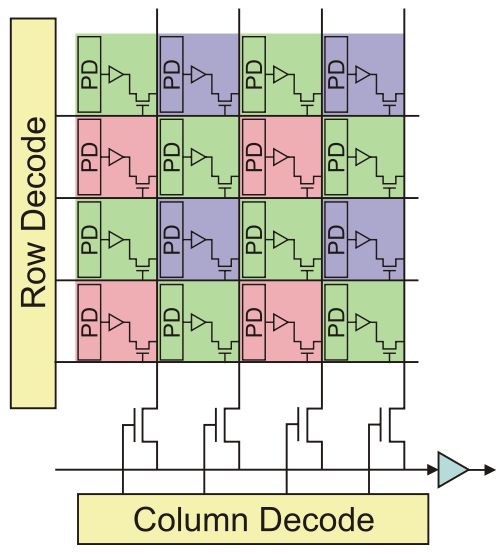
\includegraphics[width=.6\linewidth,keepaspectratio]{figures/background/cmos.png}
	\caption{CMOS array}
	\label{fig:cmosarray}
\end{figure}
\subsubsection{Microbolometers}
Both CCD arrays and CMOS arrays only capture visible light.
%
A microbolometer, on the other hand, measures the power in the infrared by exposing a thermistor\anote{thermistor} to the incident light.
%
\begin{figure}[b]
	\center
	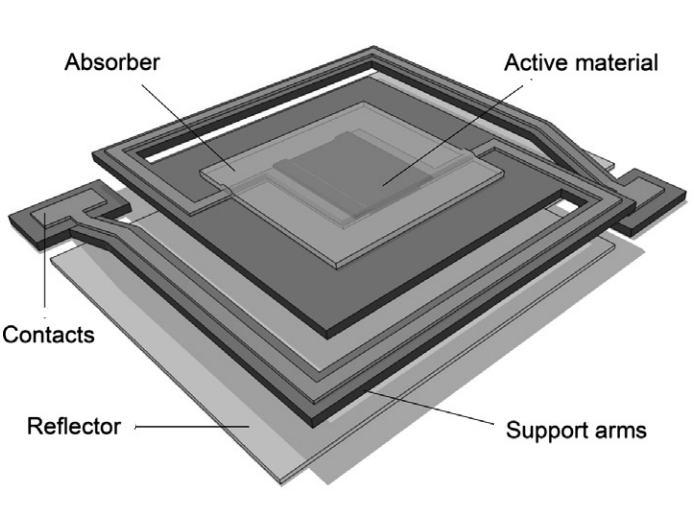
\includegraphics[width=.7\linewidth,keepaspectratio]{figures/background/microbolometer2.png}
	\caption{Bridge structure of Honeywell microbolometer\cite{KESIM2014245}}
	\label{fig:microbolometer}
\end{figure}
%
Since a thermistor's resistance changes as a function of its temperature, a key issue in the design of a microbolometer is the thermal isolation of the thermistor.
%
With the maturation of micro-machining techniques (such as for MEMS\anote{mems} devices) over the last some years, two level microbolometers consisting of a thermo-sensitive component suspended above (and insulated from) silicon have been built (see figure~\ref{fig:microbolometer}).
%
These pixel packages are evacuated and therefore have good conduction, convection, radiation heat transfer properties.
%
The actual thermo-sensitive component consists of a thermistor, an absorber (which aids in transfer of heat to the thermistor), and a reflector that creates a Fabry–Pérot optical cavity\anote{fabryperot} (typically ${\sim}\lambda/4$\cite{bolometer}) that traps the infrared light.
%
Typical materials for the thermistor are vanadium oxide and amorphous silicon owing to their high temperature coefficients of resistance\cite{bolometer}, which in effect transform small changes in temperature into large changes in resistance.
%
Measurements of the thermistor are performed by a read-out integrated circuit adjacent to the bridge in the silicon substrate.
%
All told microbolometers are designed much differently from either CCD or CMOS arrays.
%
It is as a result of this fact that high-resolution infrared cameras are not available.

Across all of these imaging systems there are ample avenues for the introductions of the kinds of errors that degrade image quality and across all of these imaging systems there are structures that impose limitations on resolving power.
%
With that in mind we now proceed to formalizing the problem of super-resolution.

\subsection{Mathematical notation}\label{subsec:notation}
Upper case plain latin $X, Y$ each denote channel $\times$ row $\times$ column \textit{tensors}\anote{tensor} representing LR and HR images respectively, with $(0, 0,0)$ corresponding to the top left corner of the first channel of image.
%
Often for the sake of simplicity we consider greyscale images, in which case we omit the channel dimension.
%
Lower case plain latin $x, y$ denote LR and HR \textit{patches}\anote{patch} respectively.
%
$D, H, F, G$ variously refer to functions that operate on images.
%
Bolded uppercase latin $\bm{X}, \bm{Y}$ are reserved for batches of images, i.e. batch size $\times$ channel $\times$ row $\times$ column tensors with $(0, 0, 0,0)$ corresponding to the top left corner of the first channel of first image in the batch.
%
Bolded lower case denote $\bm{x}, \bm{y}, \bm{z}$ etc. denote conventional column or row vectors.
%
Unless otherwise specified $\left\| \cdot \right\|$ is the $L_2$ norm.

\subsection{Imaging model}\label{subsec:imaging-model}

Figure~\ref{fig:bertrand} shows a conceptual model of the imaging process as carried out by an imaging system.
%
The input to the system is a natural scene that is in effect sampled by the imaging system.
%
In the idealized case the sampling is done at (or above) the Nyquist rate and no aliasing occurs.
%
In practice there is noise and loss introduced at every step of the process: atmospheric turbulence plays a role at large distances, motion produces multiple views of the same scene but also induces blur, imperfections of the lenses further blur the image, and finally down-sampling by the sensor elements into pixels produces aliasing artifacts\anote{ccd}.
%
The noisy, blurry, down-sampled images are then further degraded by sensor noise.
%
Each such image we call an LR sample.
\begin{figure*}
    \centering
    \begin{adjustbox}{width=\textwidth}
        \begin{tikzpicture}[auto]
            \tikzstyle{terminal} = [rectangle, draw, text width=5em, text centered, minimum height=4em]
            \tikzstyle{block} = [rectangle, draw, fill=gray!20, text width=6em, text centered, rounded corners, minimum height=4em]
            \tikzstyle{line} = [draw, -latex']
            \tikzstyle{sum} = [circle, draw]

            \node[inner sep=0pt] (bertrand) {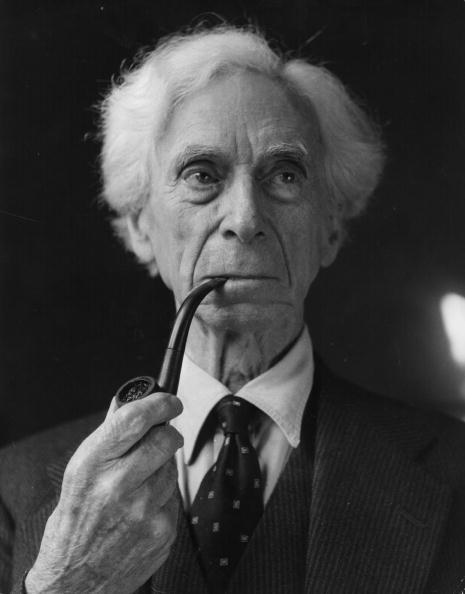
\includegraphics[width=.15\textwidth]{figures/bertrand.png}};
            \node [above = of bertrand] (scene) {Scene};

            \node[sum, right = of bertrand] (sum1) {$+$};
            \node [block, below = of sum1] (atmo-noise) {Atmospheric noise};

            \node [block, right = of sum1] (motion) {Translation, Rotation, Aspect};
            \node [above = of motion] {Motion};

            \node [inner sep=0pt, right = of motion] (motion-output) {};

            \node[inner sep=0pt, below = of motion-output] (bertrand-motion) {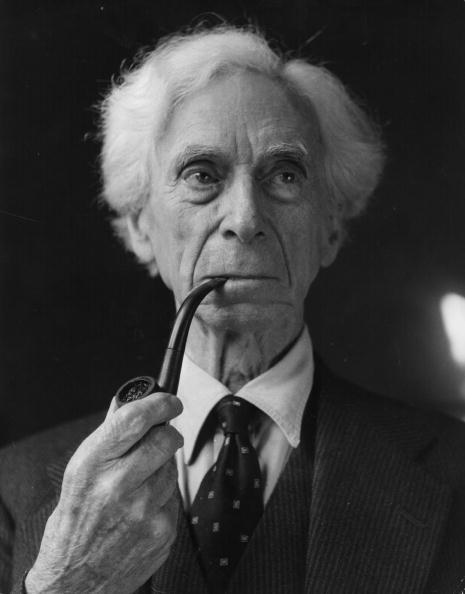
\includegraphics[width=.15\textwidth]{figures/bertrand.png}};
            \node[inner sep=0pt, below = of motion-output, xshift=2mm, yshift=-2mm] {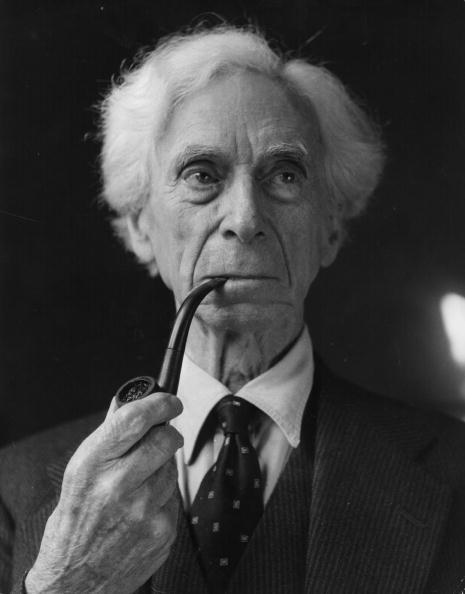
\includegraphics[width=.15\textwidth]{figures/bertrand.png}};
            \node[inner sep=0pt, below = of motion-output, xshift=4mm, yshift=-4mm] {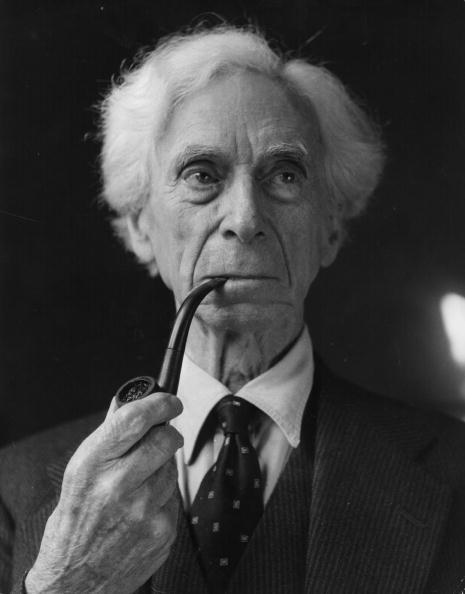
\includegraphics[width=.15\textwidth]{figures/bertrand.png}};
            \node[inner sep=0pt, below = of motion-output, xshift=6mm, yshift=-6mm] {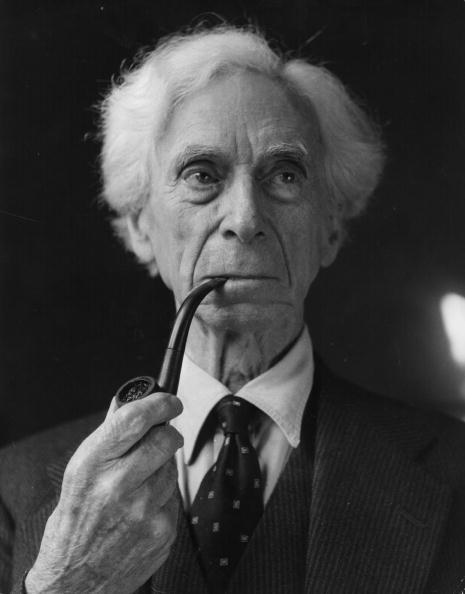
\includegraphics[width=.15\textwidth]{figures/bertrand.png}};

            \node [block, right = of motion-output] (blur) {Optical, Motion};
            \node [above = of blur] {Blur};
            \node [inner sep=0pt, right = of blur] (blur-output) {};

            \node[inner sep=0pt, below = of blur-output] (bertrand-blur) {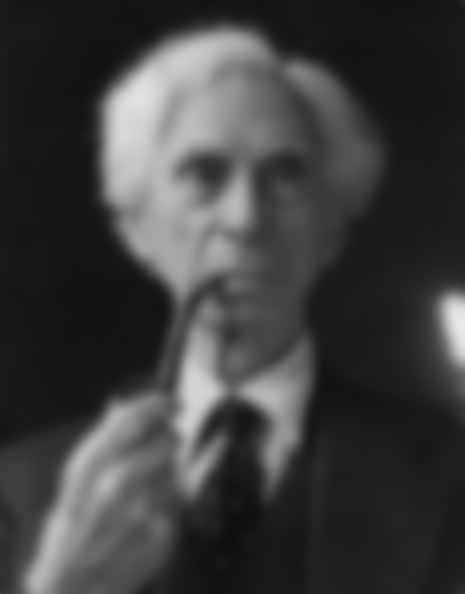
\includegraphics[width=.15\textwidth]{figures/bertrand-blur.png}};
            \node[inner sep=0pt, below = of blur-output, xshift=2mm, yshift=-2mm] {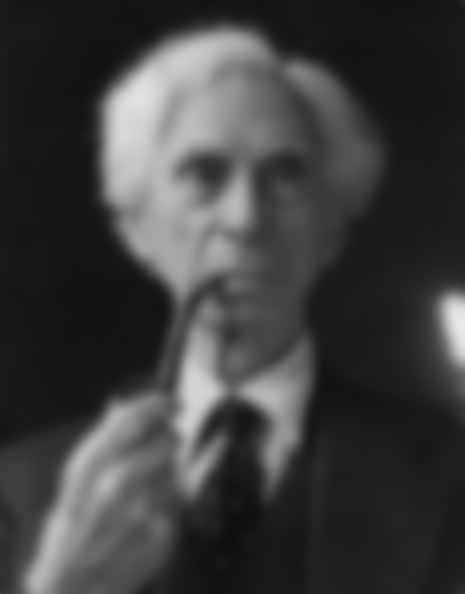
\includegraphics[width=.15\textwidth]{figures/bertrand-blur.png}};
            \node[inner sep=0pt, below = of blur-output, xshift=4mm, yshift=-4mm] {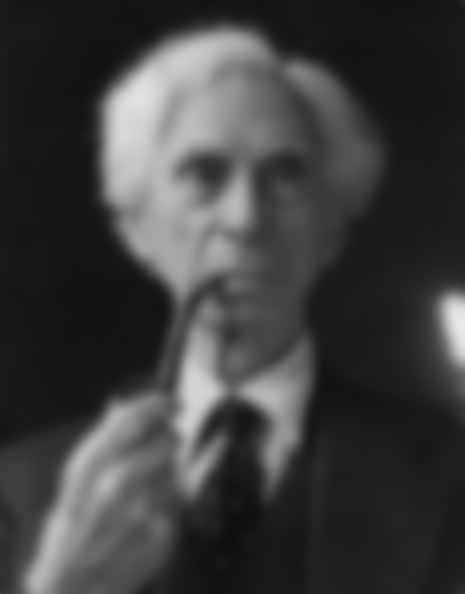
\includegraphics[width=.15\textwidth]{figures/bertrand-blur.png}};
            \node[inner sep=0pt, below = of blur-output, xshift=6mm, yshift=-6mm] {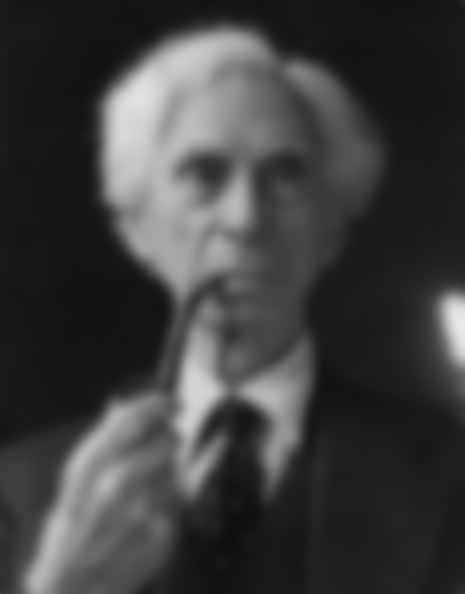
\includegraphics[width=.15\textwidth]{figures/bertrand-blur.png}};

            \node[block, right = of blur-output] (downsample) {Quantization, Pixel-binning};
            \node [above = of downsample] {Down-sampling};

            \node[sum, right = of downsample] (sum2) {$+$};
            \node [block, below = of sum2] (sensor-noise) {Sensor noise};

            \node[inner sep=0pt, right = of sum2] (bertrand-blur-noise) {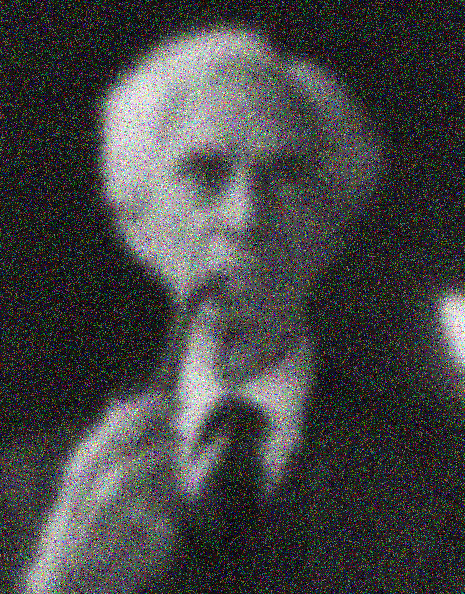
\includegraphics[width=.1\textwidth]{figures/bertrand-blur-noise.png}};
            \node[inner sep=0pt, right = of sum2, xshift=2mm, yshift=-2mm] {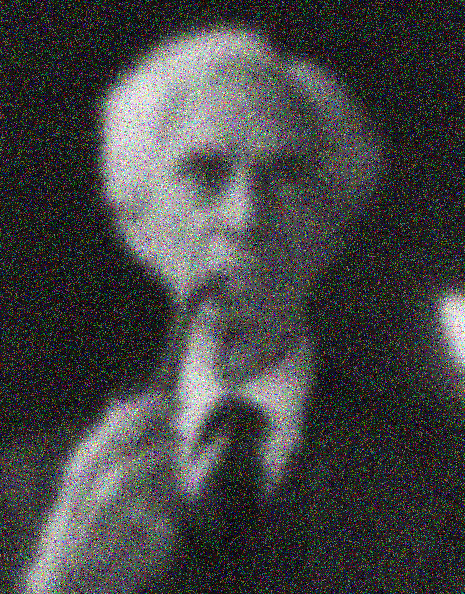
\includegraphics[width=.1\textwidth]{figures/bertrand-blur-noise.png}};
            \node[inner sep=0pt, right = of sum2, xshift=4mm, yshift=-4mm] {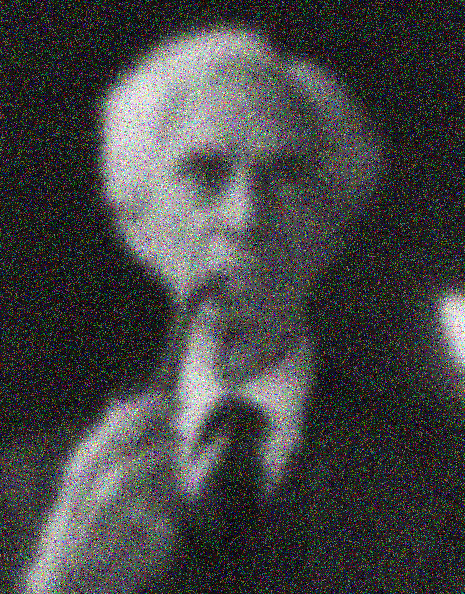
\includegraphics[width=.1\textwidth]{figures/bertrand-blur-noise.png}};
            \node[inner sep=0pt, right = of sum2, xshift=6mm, yshift=-6mm] {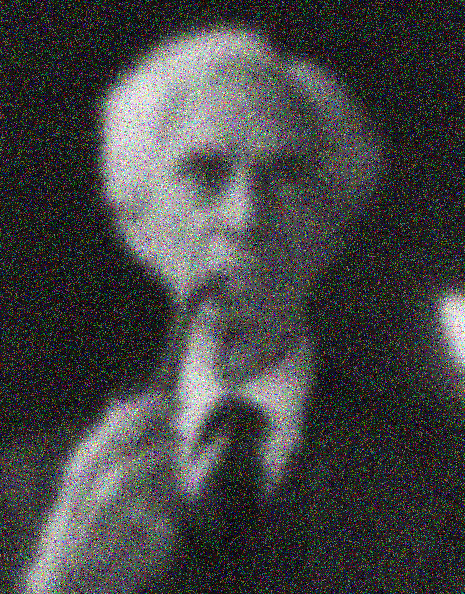
\includegraphics[width=.1\textwidth]{figures/bertrand-blur-noise.png}};
            \node [above = of bertrand-blur-noise, text width=5em] (lr-output) {Low-resolution images};

            \draw[-] (bertrand) edge (sum1);
            \draw[->] (sum1) edge (motion);
            \draw[->] (atmo-noise) edge (sum1);

            \draw[->] (motion) edge (blur);
            \draw[->] (motion-output) edge (bertrand-motion);

            \draw[->] (blur) edge (downsample);
            \draw[->] (blur-output) edge (bertrand-blur);
            \draw[->] (sensor-noise) edge (sum2);
            \draw[-] (downsample) edge (sum2);
            \draw[->] (sum2) edge (bertrand-blur-noise);
        \end{tikzpicture}
    \end{adjustbox}
    \caption{The imaging model illustrating the relationship between a scene and final low-resolution images due to noise, motion, blur, and sampling.}
    \label{fig:bertrand}
\end{figure*}

Let $Y$ denote an idealized HR image of the scene from some fixed vantage point and assume the imaging system collects $K$ LR samples $\Xk$ of $Y$.
%
Formally the $\Xk$ are related to $Y$ by
\begin{equation}
	\Xk = (D \circ H_k \circ A_k) (Y) + \varepsilon_k
	\label{eqn:imagingmodel}
\end{equation}
where for the $k$th LR sample, $A_k$ (of $K$) is the operator representing motion, $H_k$ represents the blur operator, $D$ represents the down-sampling operator (constant in time since it's typically a digital component of the imaging system), and $\varepsilon_k$ represents the composite noise (environment and sensor noise).

\subsubsection{Motion}

In the case of MISR, high-resolution images are constructed by exploiting distinct scene data among multiple low-resolution images.
%
Such distinct data are produced by the relative motion of the imaging system and the scene and therefore precise and accurate image \textit{registration}\anote{registration} is paramount.
%
Successful registration is effected by producing a transformation $f$ that maps pixels at coordinates $(x',y')$ in sample $\Xkone$ to coordinates $(x,y)$ in sample $X_j$
\begin{equation}
	\Xkone(f(x', y')) = X_j(x,y)
	\label{eqn:registration}
\end{equation}
where we use index $j$ to indicate the possibility of registering all samples relative to a fixed reference image (e.g. $j=0$ the first sample) or successive/relative registration (i.e. with $j=k$).
%
While image registration is already challenging in the various domains where samples are treated as canonical, such as remote sensing and medical imaging, in SR it is further complicated by the fact that the images to be registered are assumed uncertain.
%
Therefore, in principle, image registration and super-resolution cannot be decoupled, since image registration accuracy would be improved by operating on the estimated HR images;
%
Hardie \etal~\cite{Hardie1997} use a Bayesian framework to jointly estimate image registration parameters and the high-resolution image\cite{Hardie1997}.
%
Alternatively one can marginalize over the HR image and estimate the registration parameters using maximum-likelihood estimation (MLE) (see section~\ref{subsubsec:gaussianprocess}).

\subsubsection{Blur}

We now consider the challenges and nuances of estimating blur.
%
In general the optical transfer function (OTF) characterizes the blur of an imaging system\anote{otf}.
%
We factor the OTF into three components:
\begin{equation}
	H(u, v) = H_{\text{diff}}(u,v) H_{\text{abr}}(u,v) H_{\text{int}} (u,v)
\end{equation}
where $u,v$ are horizontal and vertical spatial frequencies respectively (measured in cycles/mm), $H_{\text{diff}}$ is blur due to diffraction, $H_{\text{abr}}$ is blur due to lens aberrations, and $H_{\text{int}}$ is blur due to imaging sensor shape (obtained by taking the Fourier transform of the shape an individual sensor in the imaging array).
%
Blur due to diffraction in most imaging systems is due to diffraction through a circular aperture\cite{goodman2005introduction}:
\begin{equation*}
	H_{\text{diff}}(u,v) =   \begin{cases}
		\frac{2}{\pi} \left(\frac{1}{\cos(\tau)} - \tau \sqrt{1-\tau^2}\right) & \text{if } \tau < 0 \\
		0                                                                      & \text{otherwise}
	\end{cases}
\end{equation*}
where $\tau = \rho/\rho_c$, $\rho=\sqrt{u^2 +v^2}$, $\rho_c = 1/\lambda N$ is the radial cutoff frequency of the aperture, $N$ is the f-number\anote{fnumber} of the optics, and $\lambda$ is the wavelength of light being diffracted.
%
This is in fact the filter that produces the Airy pattern and therefore informs sensor array spacing in order to avoid aliasing.
%
Wavelength independent blurring due to aberrations can be induced by various imperfections in the lenses such as spherical aberration, comatic aberration\anote{coma}, or astigmatism. Furthermore, dispersion\anote{dispersion} blurs particular wavelengths of light. A good model for all of these effects is\cite{10.1117.12.946501}:
\begin{equation*}
	H_{\text{abr}}(u,v) =   \begin{cases}
		1-\left(\frac{25}{65}\right)^2 \left(1-4\left(\tau - \frac{1}{2}\right)\right)^2 & \text{if } \tau < 0 \\
		0                                                                                & \text{otherwise}
	\end{cases}
\end{equation*}
Figure~\ref{fig:mtf} shows an example OTF for an imaging system with a sensor spacing of 0.050 mm and therefore sampling frequency of 20 cycles/mm and $\rho_c = 83.3~\text{cycles}/\text{mm}$ ($F=3$ and $\lambda = 4\mu\text{m}$ i.e. near infrared).
%
Notice that $\rho_c$ is much greater than the Nyquist rate ($\frac{1}{2} \times 20~\text{cycles}/\text{mm} = 10~\text{cycles}/\text{mm}$) and therefore many frequencies that are within the radial cutoff frequency will be aliased.
%
This in particular can be mitigated by effectively increasing sampling rate using MISR.
%
Notice also that like a typical transfer function the OTF is not flat and therefore attenuates high spatial frequencies.
%
Simply applying gain to the image wouldn't solve the attenuation problems because of aliasing, but likewise this can be resolved after the effective sampling rate is increased using MISR.
\begin{figure}
	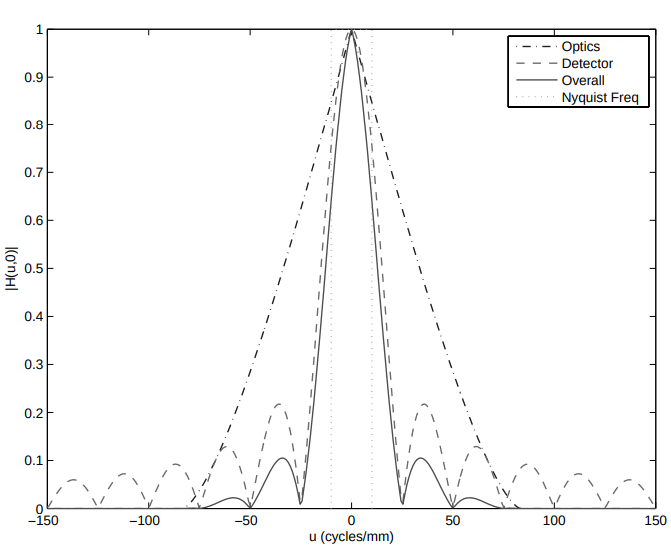
\includegraphics[width=\linewidth,keepaspectratio]{figures/background/mtf.png}
	\caption{OTF magnitude cross-section for\cite{milanfar2017super}}
	\label{fig:mtf}
\end{figure}

The challenge of super-resolution is to solve the inverse problem of finding $Y$ from one or several $\Xk$.
%
In general, since $A_k, H_k, D_k$ are highly degenerate functions, the corresponding inverse problems are ill-posed without regularization and conditioning.
%
The techniques that have been brought to bear on the problem range from interpolation to statistical estimation to example based learning.


    \section{Classical Algorithms}\label{sec:classical-algorithms}
    \subsection{Interpolation}\label{subsec:interpolation}

Suppose that $H_k$ is linear spatial\anote{lsi} and time invariant.
%
Suppose further that $A_k$ is affine.
%
Then $H \coloneqq H_k$ commutes with $A_k$\cite{meladcommute} and eqn.~\eqref{eqn:commuteimagingmodel} becomes
\begin{equation}
	\label{eqn:commuteimagingmodel}
	\begin{split}
		\Xk &= (D \circ A_k \circ H) (Y) + \varepsilon \\
		&= (D \circ A_k) (H(Y)) + \varepsilon \\
		&= (D \circ A_k) (V) + \varepsilon
	\end{split}
\end{equation}
%
where $V \coloneqq H(Y)$.
%
This naturally suggests interpolation in order to recover $V$ (since $\Xk$, in this framing, is simply shifted samples of $V$).
%
Note in this context we use interpolation very broadly, i.e. to connote filling in missing values using neighboring (in some sense --- not necessarily geometrically) values.
%
\begin{figure}
	\centering
	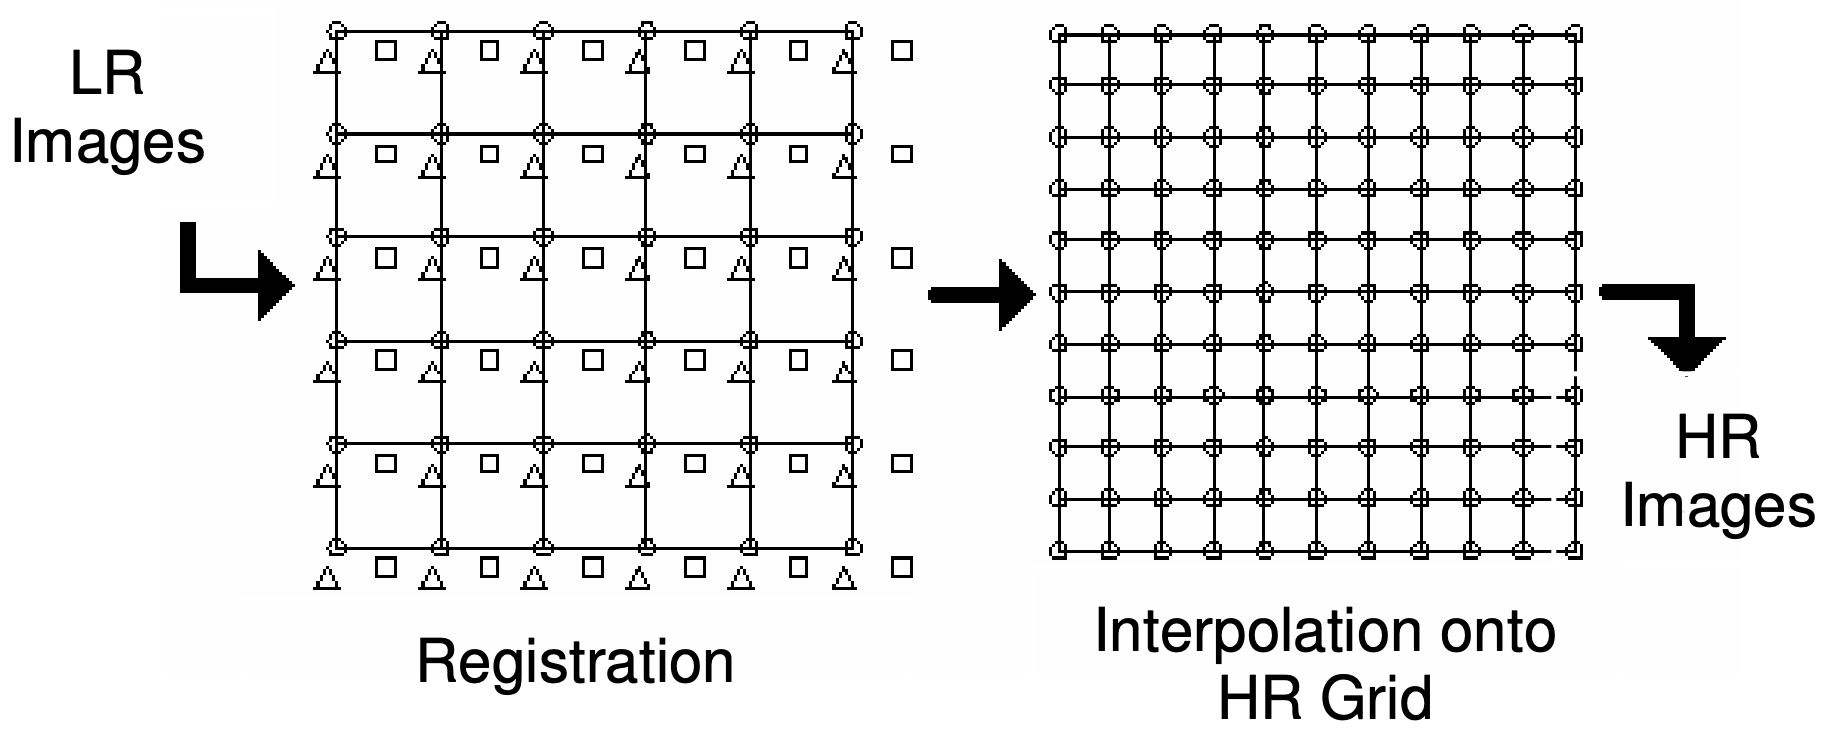
\includegraphics[width=\linewidth,keepaspectratio]{figures/classical/hrgrid.png}
	\caption{LR image registration on an HR grid\cite{Lin}}
	\label{fig:hrgrid}
\end{figure}
This class of techniques proceed by first registering images on a high resolution grid (see figure~\ref{fig:hrgrid}) then interpolating at the "missing" pixels in the HR grid to recover $V$, and finally denoising and deconvolution (of $H$) to recover $Y$.
%
Since in general consecutive $\Xk$ have non-uniform shifts (relative to $X_1$) the interpolation is non-uniform and improvisations on this theme use various weighting schemes for adjacent LR pixels\anote{lrpixel}.

For example Alam \text{et al.}\cite{Alam2000} uses weighted nearest neighbors: for every pixel to be interpolated the three nearest pixels are weighted inversely by their distance (according to HR grid distance) and then their weighted sum is assigned to that pixel.
%
This non-uniform interpolation is then followed by application of a Wiener filter whose design is informed by the OTF of the particular imaging system they study (which they do not estimate i.e. they assume they can model accurately).
%
\subsubsection{Delaunay Triangulation}

\begin{figure}
	\centering
	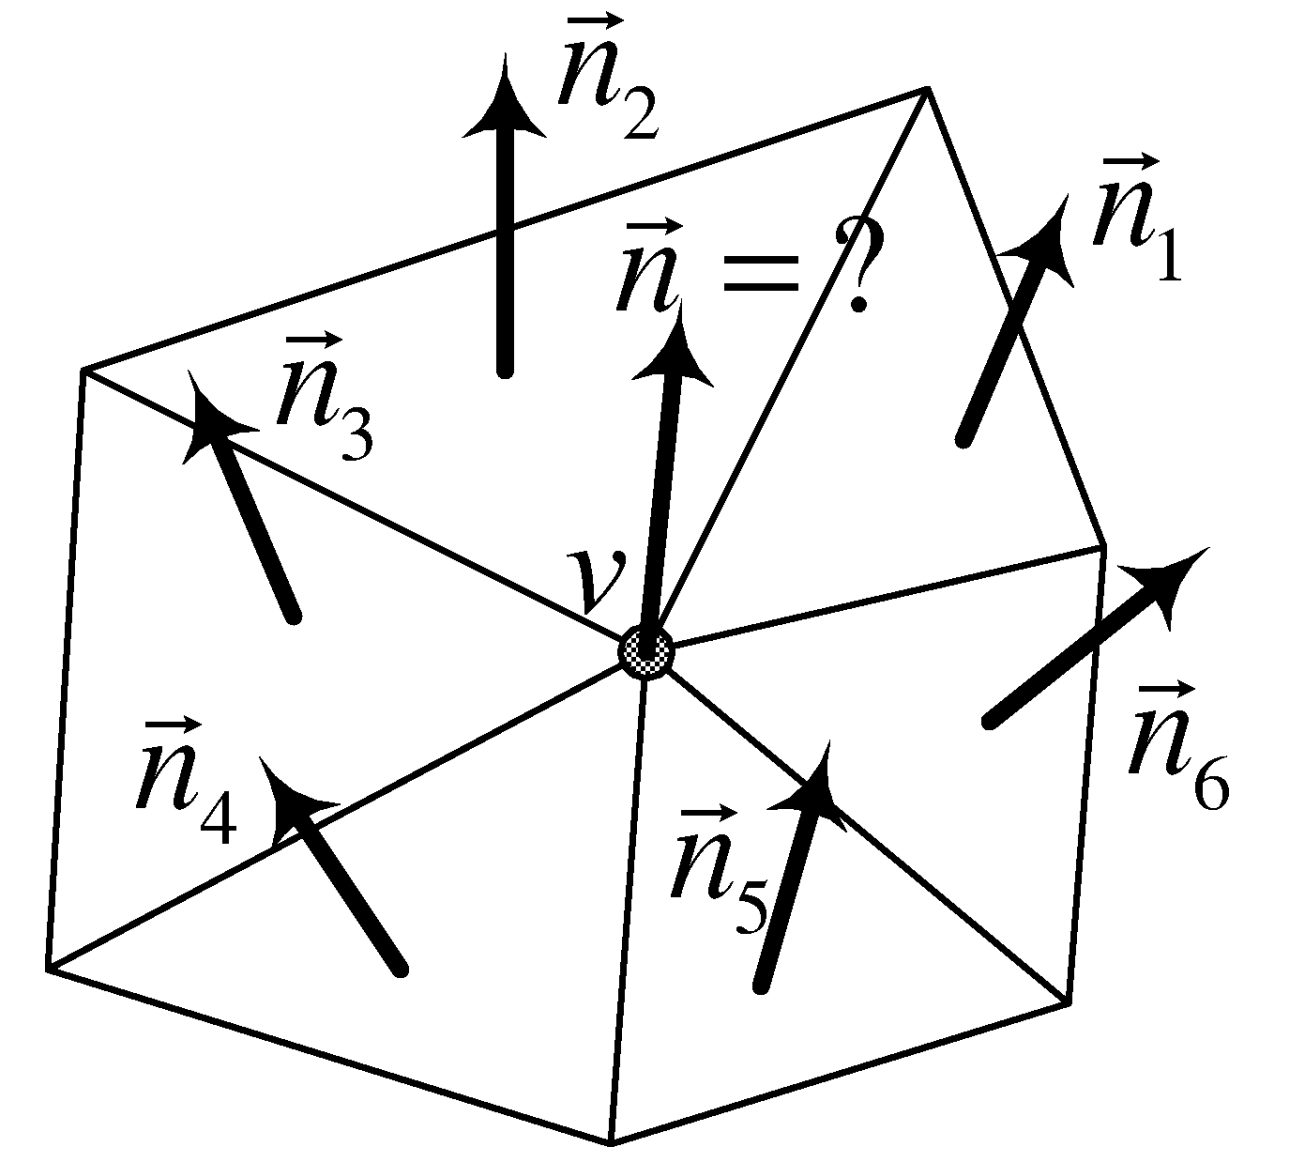
\includegraphics[width=.7\linewidth]{figures/classical/delauney.png}
	\caption{Delaunay triangulation for fitting splines at LR pixels\cite{Lertrattanapanich}. $v$ is an LR pixel. Note that $v$ is at $z$ equal to the pixel value}
	\label{fig:delauney}
\end{figure}
Lertrattanapanich \text{et al.}\cite{Lertrattanapanich} base their algorithm on interpolants which require knowledge of gradients (e.g. splines) and mediate the non-uniform sampling by using a weighted average (by area) of those gradients in adjacent Delaunay cells; to be precise they produce a Delaunay triangulation of all LR pixels and compute the gradients (see figure~\ref{fig:delauney}) according to
\begin{align*}
	\vec{n} = \sum_{i=1}^m \frac{B_j \vec{n_j}}{B}   & \text{ where } B=\sum_{i=1}^m B_i                              \\
	\frac{\partial z}{\partial x} = -\frac{n_x}{n_z} & \text{ and }  \frac{\partial z}{\partial y} = -\frac{n_y}{n_z}
\end{align*}
where $B_i$ is the area of the $i$th Delaunay cell.
%
Unfortunately this intricate solution is not robust to noise in real images.
\subsubsection{Wiener Filter}
A more sophisticated method for non-uniform interpolation uses parametric models for the auto-correlation between LR pixels and the cross-correlation between LR pixels and interpolated pixels to estimate wiener filter weights\cite{wiener}.
%
These weights are then used to average nearby pixel values.
%
The algorithm operates on a sliding \textit{estimation window} whose dimensions $D_x, D_y$ are chosen such that the effective sampling rate exceeds the Nyquist rate for a given $\rho_c$.
\begin{figure}
	\centering
	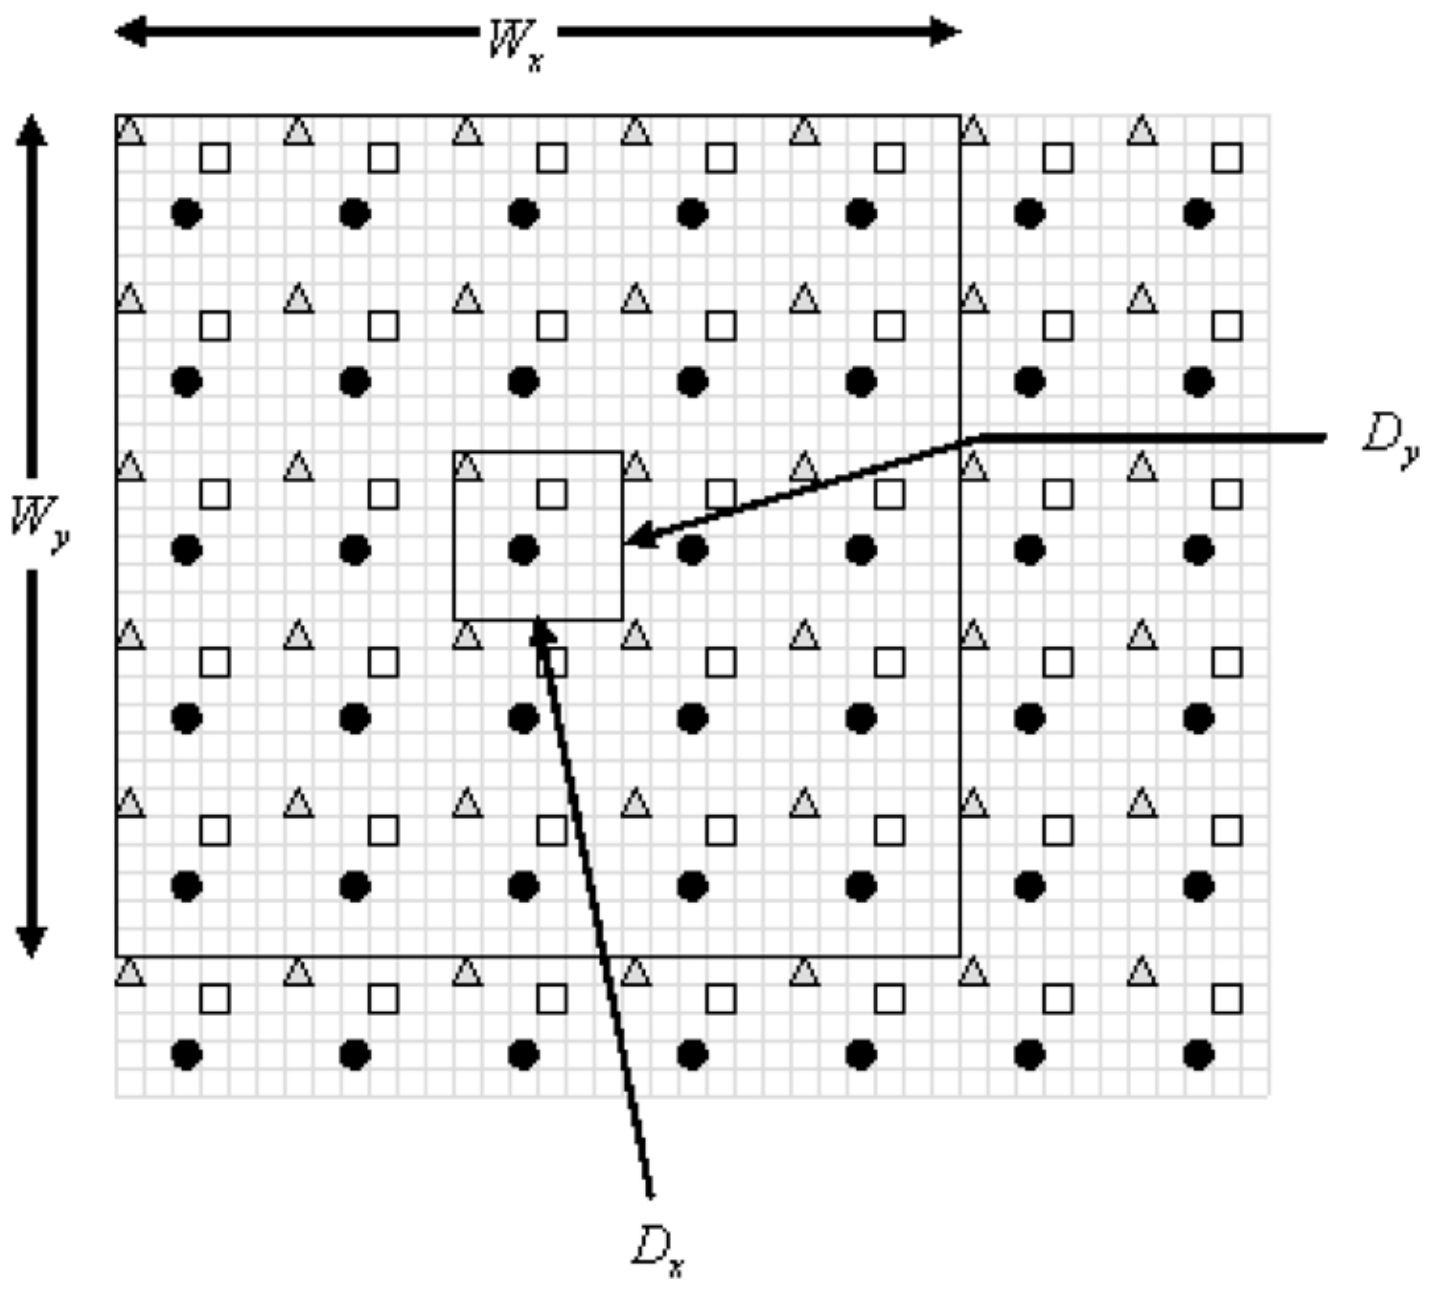
\includegraphics[width=.7\linewidth]{figures/classical/wiener.png}
	\caption{Wiener filter super resolution estimation window of dimension $D_x \times D_y$ and observation window of dimension $W_x \times W_y$\cite{wiener}}
	\label{fig:wiener}
\end{figure}
The pixel values for the estimation window are a function of the wiener filter weights of nearby LR pixels within an \textit{observation window} whose dimensions $W_x, W_y$ are an integer multiple of $D_x, D_y$ (see figure~\ref{fig:wiener}).
%
The weights $\bm{w}$ are defined as the solution to the minimum mean squared error (MMSE) filter problem, i.e. the finite impulse response (FIR) wiener filter:
\begin{equation}
	\bm{w} = R^{-1}\bm{p}
\end{equation}
where $R$ is the auto-correlation of the LR pixels in the observation window and $\bm{p}$ is the cross-correlation between the pixels to be estimated and the LR pixels.
%
Then $R$ and $\bm{p}$ are both constructed by sampling a parametric model that weights pixels in the observation window according to distance:
%
$R$ is constructed by sampling from
\begin{equation}
	C_1(r) \coloneqq \sigma_{d}^2 \rho^{r} \ast G(r)
\end{equation}
and $\bm{p}$ is constructed by sampling from
\begin{equation}
	C_2(r) \coloneqq \sigma_d^2 \rho^{r} \ast G(r) \ast G(-r)
\end{equation}
In the case of $R$, $r$ is distance on the HR grid, $\sigma_d$ is related to the empirical variance of all LR pixels in a given observation window and $G(r)$ is a smoothing kernel (e.g. Gaussian).
%
Thus by evaluating $C_1$ for all $r = r(n_1, n_2)$ distances between LR pixels $n_1$, $n_2$ we can construct $R$.
%
Similarly for $\bm{p}$, $r = r(m, n)$ is the distance between pixel-to-be-estimated $m$ and LR pixel $n$.
%
Note that $R$ is an $N \times N$ matrix where $N = K W_x W_y/D_x D_y$, i.e. how many LR pixels there are in the observation window, and $\bm{p}$ is an $N \times 1$ column vector uniquely computed for each pixel in the estimation window.
%
The scheme is effective but suffers from issues with the spatial isotropy of the auto-correlation and cross-correlation models.
\subsubsection{Steering Kernels}
One of the most sophisticated of these non-uniform interpolation schemes employs the kernel regression framework and \textit{steering kernels} (see~\ref{fig:steering}).
%
In this context we start with all $\Xk$ registered to a common HR grid and consider pixel values $Y(\bxi)$ at pixel coordinates $\bxi \coloneqq (x_{i1},x_{i2})$ as the measured data pairs $(\bxi, Y(\bxi)$.
%
Recall that kernel regression frames the estimation problem as
\begin{equation}
	Y(\bxi) = Z(\bxi) + \varepsilon
\end{equation}
where $Z$ is the to-be-estimated \textit{regression function} that "predicts" $Y$ as a function of $\bx$.
Then the Nadaraya–Watson estimator (NWE)\cite{Nadaraya} $\hat{Z}$ for $Z$ is
\begin{equation}
	\hat{Z}(\bx) = \frac{\sum_{i=1}^{P}K(\delx)Y(\bxi)}{\sum_{i=1}^{P}K(\delx)}
	\label{eqn:kernelregression}
\end{equation}
where $P$ indexes over all pixels in the HR grid and $K$ is a \textit{kernel function} whose purpose is to decay the contribution of $\bxi$ if it's in some sense far from $\bx$.
%
Note that $\hat{Z}(\bx)$ can also be seen as a weighted filtering of $Y$.
%
\begin{figure}
	\centering
	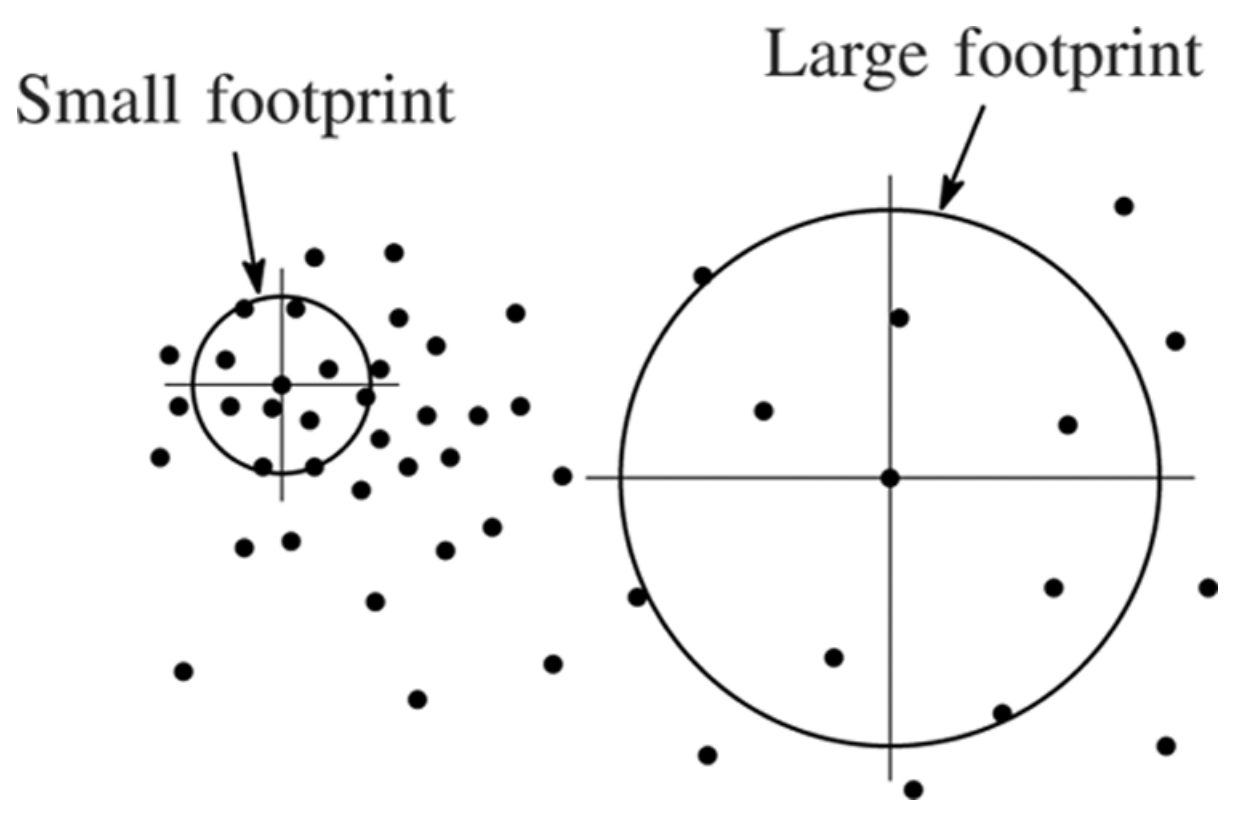
\includegraphics[width=.8\linewidth]{figures/classical/footprint.png}
	\caption{Kernel footprint as a function of sample density\cite{Takeda2007}}
	\label{fig:footprint}
\end{figure}
\begin{figure}
	\centering
	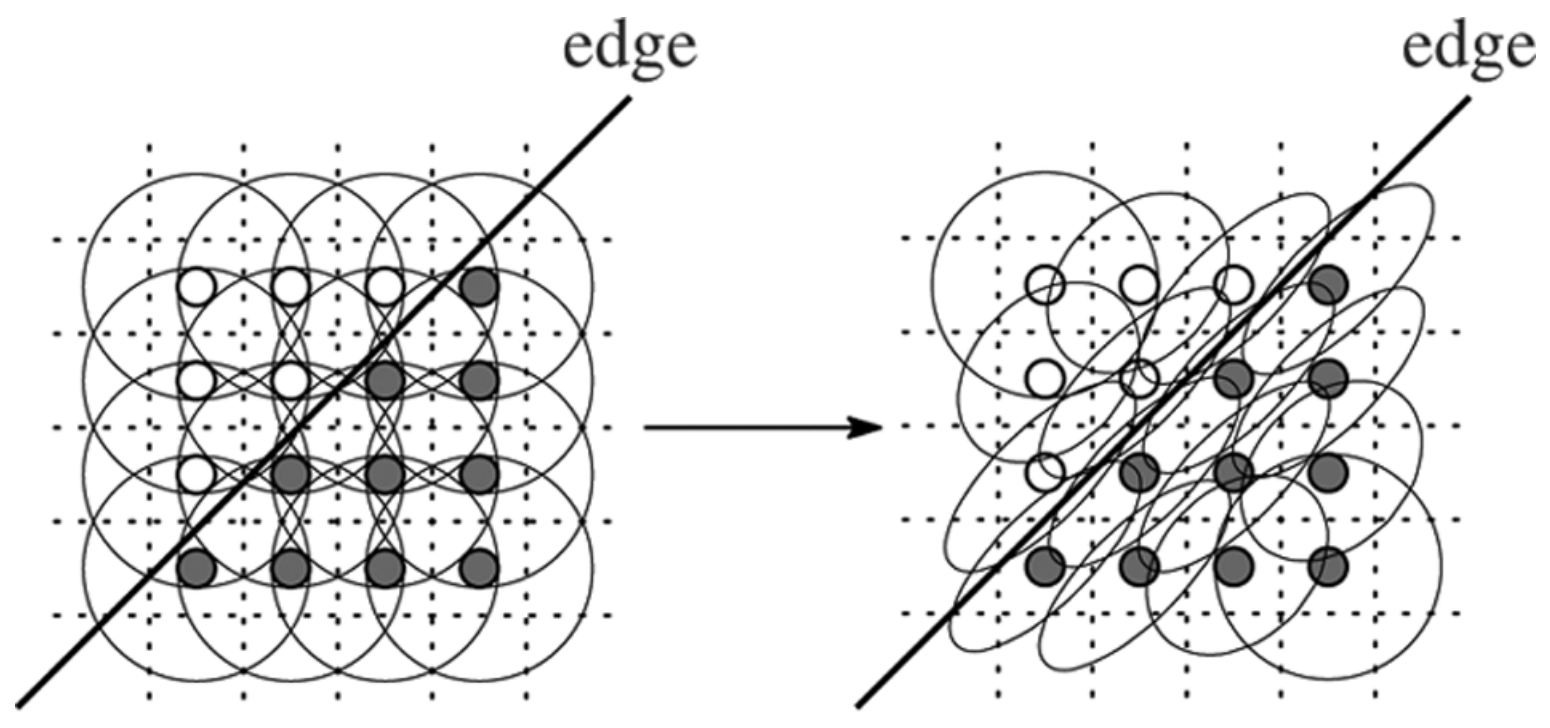
\includegraphics[width=\linewidth,keepaspectratio]{figures/classical/steering.png}
	\caption{Adapting kernel shape as a function of local directed structure\cite{Takeda2007}}
	\label{fig:steering}
\end{figure}
In conventional kernel regression $K$ might be any non-negative, symmetric, unimodal\cite{wand1994kernel} function with augmented with an additional $h$ parameter that controls the "bandwidth" or "footprint" of the kernel, i.e.
\begin{equation}
	K_h(\delx) \coloneqq \frac{1}{h}K\left( h^{-1}(\delx) \right)
\end{equation}
This bandwidth parameter $h$ can be generalized to a \textit{smoothing kernel} $H$ in order to make $K = K_H$ adaptive to the local structure of the pixels, e.g. to have larger footprints in sparsely sampled regions and have smaller footprints in densely sampled regions (see figure~\ref{fig:footprint}).
%
Ultimately though it is desirable to have kernels that can adapt to directed structure in the image, i.e. "steerable" kernels that filter strongly along an edge and weakly across an edge.
%
This is accomplished by, for example, using a Gaussian as the kernel:
\begin{equation}
	K_{H_i}(\delx) \propto \frac{\exp\left\{ -(\delx)^T H^{-1}_i (\delx) \right\}}{\sqrt{\det{H_i}}}
\end{equation}
and identifying $H_i$ with $\nabla^2 \zbxi$ (since gradients capture edge structure).
%
An estimate $\hat{H}_i$ of $\nabla^2 \zbxi$ can be obtained by looking at covariances of empirical gradients (i.e. the HR grid registered image convolved with a difference filter).
%
Unfortunately this is a naive estimate that is often rank deficient or unstable (both leading to instances where $\hat{H}_i$ isn't invertible).
%
One solution is to parameterize $H_i$:
\[
	H_i = \gamma_i U_{\theta_i} \Lambda_{\sigma_i} U_{\theta_i}^T
\]
where $U_{\theta_i}$ is a rotation matrix, $\Lambda_{\sigma_i} = \text{diag}\left( \sigma_i, \sigma_i^{-1} \right)$ is an "elongation" matrix, and $\gamma_i$ is a scaling parameter, with each of $\gamma_i, \theta_i, \sigma_i$ estimated from the data in a more robust way.
%
\subsubsection{Bilateral Kernel}
An alternative kernel is the bilateral kernel\cite{Tomasi:1998:BFG:938978.939190} that defines closeness according to geometric and radiometric distance:
\begin{equation}
	\begin{split}
		K_S(\delx) &\coloneqq \exp \left\{ -\frac{\left\| \delx \right\|^2}{2 \sigma_S^2}  \right\} \\
		K_R(\bx, \bxi) &\coloneqq \exp \left\{ -  \frac{\left\| Y(\bx) - Y(\bxi) \right\|^2}{2 \sigma_R^2} \right\} \\
		K_B(\bx, \bxi) &\coloneqq K_S(\delx)K_R(\bx, \bxi)
	\end{split}
	\label{eqn:bilateralkernel}
\end{equation}
where $\sigma_S$ parameterizes spatial distance weight and $\sigma_R$ parameterizes "radiometric" distance weight.

In general non-uniform interpolation techniques are intuitive and typically (relatively) computationally efficient but they assume an unrealistic observation model (namely that of affine motion).

\subsection{Estimation}\label{subsec:estimation}

Statistical estimation methods cast SR as an inference problem.
%
\subsubsection{Iterative Back-Projection}
One of the earliest successful SR algorithms\cite{Irani1991ImprovingRB} proposed an iterative scheme inspired by the back-projection method commonly used to reconstruct 2-D objects from 1-D projections in computer-aided tomography.
%
Recall eqn.~\eqref{eqn:imagingmodel}.
\begin{figure}
	\centering
	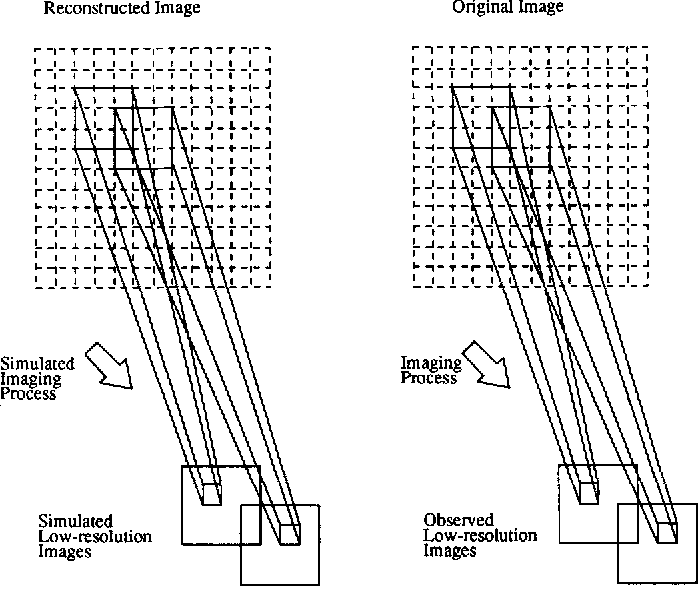
\includegraphics[width=\linewidth,keepaspectratio]{figures/classical/iterative_back_projection.png}
	\caption{Iterative back projection\cite{Irani1991ImprovingRB}}
	\label{fig:iterbackproj}
\end{figure}
%
Then the idea is to take the current estimate of the HR image $\hat{Y}^{i}$, see if after motion and down-sampling $(D \circ A_k)(\hat{Y}^i)$ it is near the LR samples $\Xk$, and add a correction when it is not (see figure~\ref{fig:iterbackproj}):
\begin{equation}
	\hat{Y}^{i+1} = \hat{Y}^i + \sum_{k=1}^K (D \circ A_k)^{-1}\left( (D \circ A_k)(\hat{Y}^i) - \Xk \right)
	\label{eqn:ibp}
\end{equation}
where $\hat{Y}^i$ is the current estimate of the blurred HR image, $(D \circ A_k)(\hat{Y}^i)$ is the projection of the current estimate to low resolution, and $(D \circ A_k)^{-1}\left( (D \circ A_k)(\hat{Y}^i) - \Xk \right)$ is the \textit{back-projection}.
%
This process iterates until convergence i.e. $\lvert (D \circ A_k)(\hat{Y}^i) - \Xk \rvert < \delta$ for some $\delta$.
%
Irani \etal\cite{Irani1991ImprovingRB} also convolve the back-projection with a smoothing kernel as a form of regularization since the estimation problem is in general ill-posed (there are many $\hat{Y}^{i}$ that will project down to a pixel-distance neighbor of $\Xk$).
%
It can be shown\cite{Elad1996} that for $\varepsilon_k$ distributed $(0, R_k)$-Normal, $\hat{Y}$ is none other than the maximum likelihood MLE for $Y$.
%
We can see this by recognizing that eqn.~\eqref{eqn:ibp} is just the Richardson iterative\cite{Anderssen:1972:RNM:891962} solution to
\begin{equation}
	L(Y) = \frac{1}{2} \left\| \bm{X} -  \begin{bmatrix}
		D_1 \circ A_1 \\
		D_2 \circ A_2 \\
		\vdots        \\
		D_K \circ A_K \\
	\end{bmatrix}  Y  \right\|^2
	\label{eqn:l2regression}
\end{equation}
since
\begin{equation*}
	\nabla_{Y} L = 0
	\iff
	\sum_{k=1}^K (D \circ A_k)^{-1}\left( (D \circ A_k)(Y) - \Xk \right) = 0
\end{equation*}
and therefore $\hat{Y}_i \rightarrow \hat{Y}$ is the MLE (since MLE is the solution to least squares\cite{CaseBerg:01}).
%
Though this is one of the oldest SR algorithms it's recently been revisited and re-imagined as a deep neural network architecture (DNN)\cite{DBLP:journals.corr.abs-1803-02735}.
\subsubsection{Kalman Filter}
Another estimation technique employs a Kalman filter\cite{elad1999} to estimate $Y$.
%
Let $\bm{x}_k = \text{vec}(\Xk)$ be the vectorization\anote{vectorize} of $\Xk$ and $\bm{y} = \text{vec}(Y)$ likewise.
%
If we assume linear models for each of $D, A_k, H_k$ (i.e. all representable as matrices) and a well-behaved motion model (most pixels in image $\bm{x}_k$ appear in image $\bm{x}_{k-1}$) then we can image $\bm{y}$ as a sequence of images $\bm{y}_k$ related in time by
\begin{equation}
	\bm{y}_k = A'_k \bm{y}_{k-1} + \eta_k
	\label{eqn:kalmanprocess}
\end{equation}
%
where $A'_k$ is the \textit{relative} motion operator, $A'_k\bm{y}_{k-1}$ is conventional matrix-vector multiplication, and $\eta_k$ is the only source of new pixels (noise\anote{noise} distributed $(0, Q_k)$-Normal).
%
Consequently eqn.~\eqref{eqn:imagingmodel} becomes
\begin{equation}
	\bm{x}_k = DH_k\bm{y}_k + \varepsilon_k
	\label{eqn:kalmanobs}
\end{equation}
and the pair of eqns.~\ref{eqn:kalmanprocess},~\ref{eqn:kalmanobs} can be seen to constitute a linear dynamical system with $\bm{y}_k$ the state of the system, $A'_k$ the state transition, $\eta_k$ the state noise, $\bm{x}_k$ the measurement, $DH_k$ the measurement model, and $\varepsilon_k$ the measurement noise.
%
Note that the HR image conditioned on all previous LR images (measurements)
\begin{equation}
	\bm{y}_{k|s} \coloneqq \bm{y}_k|\bm{x}_1, \mathellipsis, \bm{x}_s
\end{equation}
where $s \leq k$, is a GP, with mean $\bar{\bm{y}}_{k|s} = E\left[\bm{y}_{k|s}\right]$
and covariance
\begin{equation}
	C_{k|s} \coloneqq E\left[ (\bm{y}_k - \bar{\bm{y}}_{k|s})(\bm{y}_k - \bar{\bm{y}}_{k|s})^T  \right]
\end{equation}
%
By definition the MMSE $\hat{\bm{y}}_{k|s}$ of $\bm{y}_{k|s}$ is $\bar{\bm{y}}_{k|s}$ and therefore $C_{k|s}$ is the covariance of the error of the estimate $\hat{\bm{y}}_{k|s}$.
%
The Kalman filter proceeds in two steps: an \textit{a priori} (before measurement) prediction step and an \textit{a posteriori} (after measurement) update step.
%
The prediction step iterates on the estimate (and its covariance) given all previous measurements:
\begin{align}
	\hat{\bm{y}}_{k|k-1} & = A'_k \hat{\bm{y}}_{k-1|k-1}     \\
	C_{k|k-1}            & = A'_k C_{k-1|k-1} (A'_k)^T + Q_k
\end{align}
This can be seen as a one-step propagation of the estimate "in the direction" of the previous measurement.
%
Then the update step incorporates new information from a measurement:
\begin{align}
	\hat{\bm{y}}_{k|k} & = \hat{\bm{y}}_{k|k-1} + K_k(\bm{x}_k - DH_k\hat{\bm{y}}_{k|k-1} ) \\
	C_{k|k}            & = (I - K_k DH_k)C_{k|k-1}
\end{align}
where the \text{Kalman gain}
\begin{equation}
	K_k \coloneqq \frac{C_{k|k-1}(DH_k)^T}{DH_k C_{k|k-1} (DH_k)^T + R_k }
\end{equation}
weights the contribution of the prediction and the measurement\anote{kalmanprediction}.
%
Note that in the Kalman framework $D, H_k, A'_k, R_k, Q_k$ are all assumed to be known.
%
In Elad \etal\cite{elad1999} the assumption is $D, H_k, R_k$ are known functions of camera parameters, $A'_k$ can be estimated by an image registration algorithm and $Q_k$ can be approximated:
\begin{equation}
	Q_k \approx \alpha_k A'_k C_{k|k} (A'_k)^T
\end{equation}
where $\alpha_k$ is chosen such that the approximation upper-bounds the true $Q_k$.
%
They comment that this stronger auto-correlation for $\bm{y}_k$ adds "pseudo-noise" to the system and biases the Kalman filter to "rely" more on the measurements than the state transition model.
\subsubsection{MAP Estimation}
SR can also be posed as a Bayesian maximum a posterior (MAP) estimation problem.
%
Let $\bm{H} \coloneqq \left( H_1, \mathellipsis, H_k \right)$ be the vector of blur operators applied to $Y$ in order to produce $\bm{X}$ and similarly $\bm{A}$.
%
Then
\begin{align}
	\hat{Y} & = \underset{Y}{\text{argmax}}~P\left( Y \middle| \bm{X} \right) \nonumber                                                                                                \\
	        & = \underset{Y}{\text{argmax}} \int_{D, \bm{H}, \bm{A}} P\left( Y, D, \bm{H}, \bm{A} \middle| \bm{X}\right) \nonumber                                                     \\
	        & = \underset{Y}{\text{argmax}} \int_{D, \bm{H}, \bm{A}} \frac{P\left(\bm{X} \middle| Y, D, \bm{H}, \bm{A} \right)P(Y) P(D, \bm{H}, \bm{A})}{P(\bm{X})}\label{eqn:indepym} \\
	        & = \underset{Y}{\text{argmax}} \int_{D, \bm{H}, \bm{A}} P\left(\bm{X} \middle| Y, D, \bm{H}, \bm{A} \right)P(Y) P(D, \bm{H}, \bm{A}) \label{eqn:maxx}
\end{align}
where in eqn.~\eqref{eqn:indepym} we've used the independence of $Y$ and $D, \bm{H}, \bm{A}$\cite{Hardie1997} and in eqn.~\eqref{eqn:maxx} we've used that $\bm{X}$ is a constant with respect to the maximization.
%
While there exist reasonable priors for $Y$, marginalizing over $D, \bm{H}, \bm{A}$ is still difficult due to the high-dimensionality of each.
%
Therefore assuming $D, \bm{H}, \bm{A}$ can be estimated independently as $\hat{D}, \hat{\bm{H}}, \hat{\bm{A}}$, eqn.~\eqref{eqn:maxx} becomes
\begin{equation}
	\hat{Y} = \underset{Y}{\text{argmax}}~P\left(\bm{X} \middle| Y; \hat{D}, \hat{\bm{H}}, \hat{\bm{A}} \right) P(Y)
	\label{eqn:map}
\end{equation}
where the semicolon indicates $\hat{D}, \hat{\bm{H}}, \hat{\bm{A}}$ are known parameters of the conditional distribution.
%
This casts $\hat{Y}$ the standard MAP estimate of $Y$.
%
Note that an equivalent formulation of MAP maximizes the log-likelihood instead of maximizing the likelihood:
\begin{align}
	\hat{Y} & = \underset{Y}{\text{argmax}}\left[ \log\left( P\left(\bm{X} \middle| Y; \hat{D},  \hat{\bm{H}}, \hat{\bm{A}}\right) P(Y) \right) \right]  \nonumber \\
	        & =  \underset{Y}{\text{argmax}}\left[ \log{P\left(\bm{X} \middle| Y; \hat{D},  \hat{\bm{H}}, \hat{\bm{A}} \right)} + \log{P(Y)} \right]
	\label{eqn:logmap}
\end{align}
%
Various choices for $P\left(\bm{X} \middle| Y; \hat{D},  \hat{\bm{H}}, \hat{\bm{A}} \right)$ and the prior $P(Y)$ (and consequent choice of optimization strategies) characterize this class of SR techniques.
%
Again assume $D, H_k, A_k$ linear and given $\varepsilon_k$ in eqn.~\eqref{eqn:imagingmodel} distributed $(0, rI)$-Normal
\begin{equation}
	P\left(\bm{X} \middle| Y; \hat{D},  \hat{\bm{H}}, \hat{\bm{A}} \right) \propto \exp \left\{ -\frac{\left\| \bm{X} - \hat{D} \hat{\bm{H}} \hat{\bm{A}} \bm{y} \right\|^2}{2r^2} \right\}
\end{equation}
where here $\bm{X} = \left( \text{vec}(X_1), \mathellipsis, \text{vec}(\Xk) \right)$ and
\begin{equation}
	\hat{D} \hat{\bm{H}} \hat{\bm{A}} \coloneqq \begin{bmatrix}
		\hat{D} \hat{\bm{H}}_1 \hat{\bm{A}}_1 \\
		\hat{D} \hat{\bm{H}}_2 \hat{\bm{A}}_2 \\
		\vdots                                \\
		\hat{D} \hat{\bm{H}}_K \hat{\bm{A}}_K \\
	\end{bmatrix}
\end{equation}
%
After a suitable choice for the prior it can be seen that eqn.~\eqref{eqn:logmap} is just regularized regression.
%
For example when choosing a Gibbs\cite{Hardie1997} distribution as the prior, i.e.
\begin{equation}
	P(Y) \propto e^{-\alpha B(Y)}
	\label{eqn:gibbs}
\end{equation}
where $B(Y)$ is called the \textit{potential}, eqn.~\eqref{eqn:logmap} becomes
\begin{equation}
	\hat{\bm{y}} = \underset{\bm{y}}{\text{argmin}}\left[ \left\| \bm{X} - \hat{D} \hat{\bm{H}} \hat{\bm{A}} \bm{y} \right\|^2 +\lambda B(Y)\right]
	\label{eqn:minmap}
\end{equation}
where the aggregate regularization parameter $\lambda$ absorbs $\alpha$ from $P(Y)$ and $r$ from $\varepsilon_k$.
%
There are many other choices for the prior in eqn.~\eqref{eqn:logmap}, whose effect is to bias the estimator $\hat{\bm{y}}$ towards "natural" images.
%
Alternatively we can (and will) take eqn.~\eqref{eqn:minmap} as our starting point and explicitly choose the regularizer $B(Y)$.

\subsubsection{Tikhonov Regularization}

One of the simplest priors is a $(0, Q)$-Normal, where $Q$ is symmetric positive definite\anote{positivedef} (PD) and captures the covariance.
%
This corresponds to the regularizer taking the form
\begin{equation}
	B(Y) = \by ^T Q \by
\end{equation}
where $\by = \text{vec}(Y)$.
%
Since $Q$ is symmetric PD eqn.~\eqref{eqn:minmap} becomes
\begin{equation}
	\hat{\bm{y}} = \underset{\bm{y}}{\text{argmin}}\left[ \left\| \bm{X} - \hat{D} \hat{\bm{H}} \hat{\bm{A}} \bm{y} \right\|^2 +\lambda \left\| \sqrt{Q}\bm{y} \right\|^2 \right]
	\label{eqn:tikminmap}
\end{equation}
where $\sqrt{Q}$ is $U$ of the Cholesky decomposition $Q = U^T U$.
%
Equation~\ref{eqn:tikminmap} is Tikhonov regularized regression, or Ridge regression if $\sqrt{Q} = I$.
%
Letting $G = \hat{D} \hat{\bm{H}} \hat{\bm{A}}$ the closed-form solution to eqn.~\eqref{eqn:tikminmap} is
\begin{equation}
	\hat{\by} = \left( G^T G + \lambda Q \right)^{-1} G^T\bX
	\label{eqn:closedform}
\end{equation}
Nguyen \etal\cite{milanfar2001} use cross-validation to determine the regularization parameter $\lambda$ (by partitioning the pixels into a "fit" and "validate" set).
%
In general, rather than explicitly computing inverses in eqn.~\eqref{eqn:closedform}, in practice $\hat{\bm{y}}$ is found by solving the regression problem via optimization (for high-dimensional matrices optimization is faster than inversion).
%
Nguyen \etal~ use conjugate gradient descent\anote{conjugategradients} to optimize eqn.~\eqref{eqn:tikminmap}.
%
They argue that $\hat{D} \hat{\bm{H}} \hat{\bm{A}}$ is ill-conditioned\anote{illcondition} and to that end, since the convergence rate of conjugate gradients is dependent on the condition number\cite{vanderSluis1986}, propose pre-conditioners\anote{precondition} to improve the converge rate.

\subsubsection{Huber Loss and TV Loss}

An issue with the multivariate Normal prior is that it strongly enforces global smoothness, penalizing sharp edges.
%
One solution is to use Huber loss\cite{huber1964}
\begin{equation}
	L_{\delta }(a)\coloneqq {
		\begin{cases}
			a^2                                 & \text{for }\lvert a \rvert \leq \delta \\
			2 \delta \lvert a \rvert - \delta^2 & {\text{otherwise}}
		\end{cases}
	}
\end{equation}
to explicitly parameterize the penalty for gradients (i.e. high-frequency features).
%
Huber loss enforces local smoothness (since it's quadratic for $\lvert a \rvert \leq \delta$) but permits edges (since it's linear for $\lvert a \rvert > \delta$).
%
Capel \etal\cite{capel2000} implement this by composing $L_{\delta }(a)$ with a first-order gradient operator\anote{gradientoperator} as the potential in eqn.~\eqref{eqn:gibbs}.
%
Another gradient penalty that encourages sparse gradients (i.e. local smoothness and steep edges) is Total Variation (TV) norm\cite{RUDIN1992259}:
\begin{equation}
	\|u\|_{\operatorname {TV}}\,\coloneqq\int _{\Omega }\|\nabla u\|\,d\Omega
\end{equation}
where $u$ is a smooth image of bounded variation (i.e. such that the integral converges) over domain $\Omega$.
%
In the context of SR this amounts to setting
\begin{equation}
	B(Y) = TV(Y) \coloneqq \lVert \nabla Y \rVert_1
\end{equation}
%
Farsiu \etal\cite{farsiu} introduce a \textit{bilateral} TV norm
\begin{equation}
	BTV(Y) \coloneqq \sum_{k=0}^{N} \sum_{l=0}^{N} \alpha^{k + l} \lVert Y - S_x^k S_y^l Y \rVert_1
\end{equation}
where $S_x^k, S_y^l$ are shift operators (i.e. $S_x^k$ shifts $Y$ by $k$ pixels in the horizontal) and $N$ is arbitrary.
%
The bilateral TV norm factors in gradients at several scales ($Y - S_x^2 Y$ is an approximation of the horizontal gradient at twice the scale of $Y - S_x^1 Y$) and decays their contribution according to their spatial distance ($\alpha^{k+l}$ decays as a function of shift distance).
%
It can also be shown to be equivalent\cite{elad2002} to filtering $\bX$ by the bilateral kernel (see eqn.~\eqref{eqn:bilateralkernel}).

Though there are many priors (or regularizers) that have been studied none really capture natural images in all of their variation.
%
For that we need to actually learn from real data i.e. examples images.

\subsection{Example based}\label{subsec:example-based}

Example based techniques \textit{learn} a mapping from
LR patches to HR patches based on a training set and then use that mapping to predict details in new (unseen) images.

\subsubsection{Hidden Markov Random Field}

Freeman \etal\cite{freeman2002example} argues that the most important features to reconstruct are the high-frequency features.
%
Therefore they store only the correspondence between high-pass filtered, contrast-normalized versions of example LR patches and HR patches.
%
Note that they pre-process the LR images by cubic-spline interpolating to the higher pixel sampling resolution and that HR patches are sampled to overlap by one or more pixel widths at their edges.
%
Naive mosaicing of these matching HR patches produces poor results due to noise and the ill-posed nature of super-resolution.
%
\begin{figure}
	\centering
	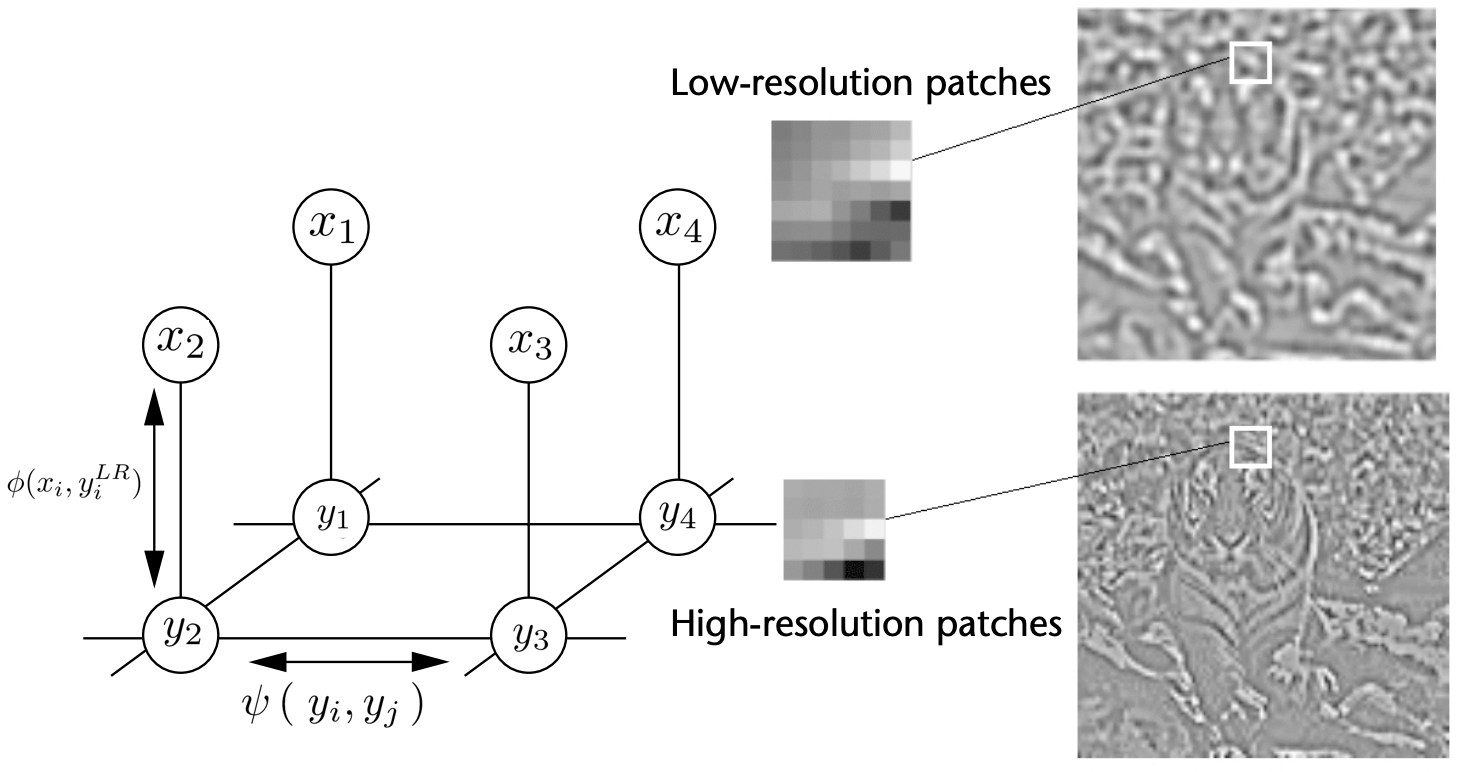
\includegraphics[width=\linewidth,keepaspectratio]{figures/classical/mrf.png}
	\caption{Hidden Markov random field modeling spatial relationships between LR patches $x_i$ and example LR patches $y_i^{LR}$ and HR patches $y_i$\cite{freeman2002example}}
	\label{fig:mrf}
\end{figure}
Their solution to this issue is using a hidden Markov random field\anote{hmrf} (HMRF) to model spatial consistency between adjacent HR patches $y_i$ and between LR-HR patch pairs $x_i, y_i$ (see figure~\ref{fig:mrf}).
%
They then compute the MAP estimate of the HMRF to obtain the smoothest assignment of HR patches: the HMRF model postulates that the conditional probability of any HR patch assignment $\by$ given observed LR patches $\bx$ is
\begin{equation}
	P\left( \by \middle| \bx \right) = \frac{1}{P(\bx)} \prod_{i\ue{} j} \psi(y_i, y_j) \prod_i \phi(x_i, y_i^{LR})
\end{equation}
where $x_i$ are observed LR patches and $y_i$ are unknown (to-be-inferred) HR patches (along with their learned-mapping example LR patches $y_i^{LR}$).
%
Note $P(\bx)$ is a normalization constant, $i\ue{} j$ indicates the product is only over adjacent HR patches, $\psi(y_i, y_j)$ encodes the compatibility of adjacent HR patches according to
\begin{equation}
	\psi(y_i, y_j) = \exp \left\{ -  \frac{\left\| y_i - y_j \right\|}{2\sigma^2} \right\}
\end{equation}
where $\left\| y_i - y_j \right\|$ is only computed on the overlapping pixels.
%
Similarly $\phi(x_i, y_i^{LR})$ encodes the compatibility between the observed LR patch $x_i$ and the example LR patch $y_i^{LR}$ corresponding to the estimated HR patch $y_i$.
%
To make the MAP computation tractable they choose only 16 candidate example LR patches $y_i^{LR}$.
%
They compute the MAP estimate using belief propagation\anote{beliefpropagation}.
\subsubsection{Nearest Neighbor Embedding}
The main problem with the direct LR-HR patch pair technique is that it requires an enormous database of patches in order for it to generalize.
%
\begin{figure}
	\centering
	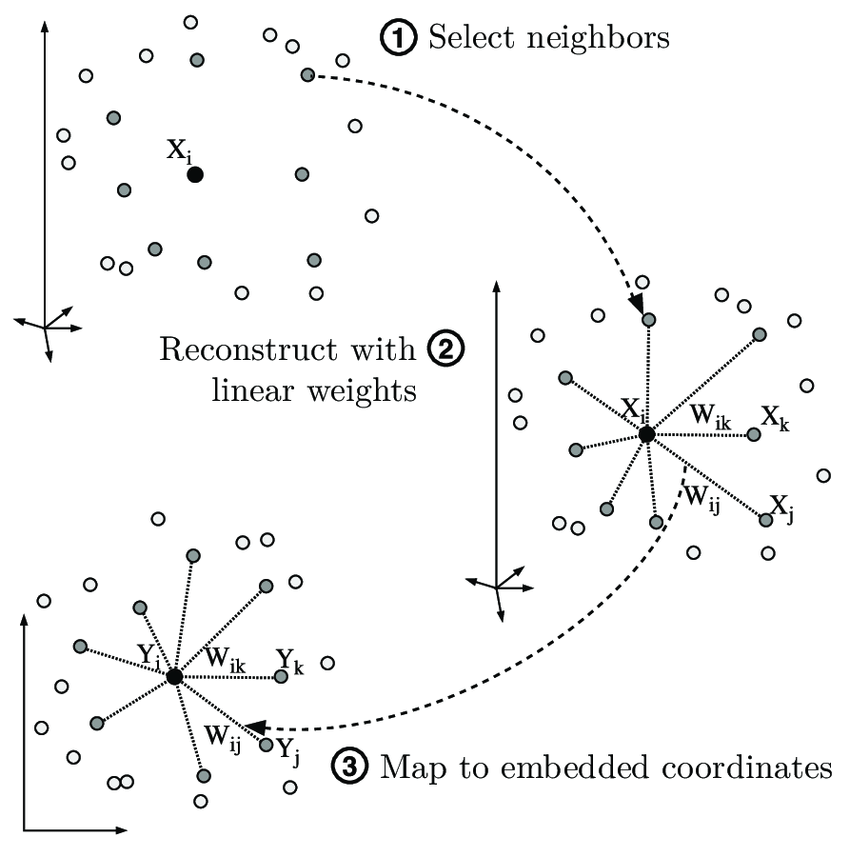
\includegraphics[width=\linewidth,keepaspectratio]{figures/classical/lle.png}
	\caption{NNE algorithm from LR patches $x_i$ to HR patches $y_i$\cite{Guillermophdthesis}}
	\label{fig:lle}
\end{figure}
Chang \etal~ remedy this problem by using ideas from a manifold\anote{manifold} learning\anote{manifoldlearning} technique called locally linear embedding\cite{saul2000introduction} (LLE) that they call nearest neighbor embedding (NNE).
%
First they imagine both the space of LR patches and HR patches as manifolds.
%
Then based on the intuition that a well-sampled smooth manifold is locally linear (i.e. an LR patch $x_i$ on the LR manifold and its neighbors $x_j, x_k, \mathellipsis$ lie in a locally linear subspace of the manifold) they characterize the local geometry.
%
One can characterize local geometry by finding convex reconstruction weights $W_{ij}$ of any $x_i$ from only its neighbors by minimizing reconstruction error, i.e.
\begin{gather}
	\hat{W} = \underset{W_{ij}}{\text{argmin}} \sum_i \left\| x_i - \sum_{x_j \in N(x_i)} W_{ij} x_j  \right\|^2 \nonumber \\
	\text{s.t.} \\
	\sum_{x_j \in N(x_i)} W_{ij} = 1 \text{ for all }i \nonumber
\end{gather}
where $N(x_i)$ is the neighborhood of $x_i$.
%
These weights $W_{ij}$ are invariant with respect to rotation, rescaling, and translation of the LR patch and its neighborhood\cite{saul2000introduction} and therefore should remain valid in an embedding space (i.e. the HR manifold) coordinate system (see figure~\ref{fig:lle}).
%
The HR patches $y_i$ in the HR manifold are then reconstructed using the same weights, i.e.
\begin{equation}
	y_i = \sum_{x_j \in N(x_i)} W_{ij} y_j
\end{equation}
%
Note that neighboring patches in HR space are constrained to overlap and in fact the neighborhoods are computed using gradient features of the LR and HR patches rather than the raw patches (they argue that this is what allows for better generalization i.e. much smaller patch databases).
\subsubsection{Sparse Coading}
The NNE approach suffers from its own issues; using a fixed number of nearest neighbors results in blurring (due to over-fitting or under-fitting).
%
Yang \etal\cite{yang2008} resolve this issue by using sparse coding (SC) as a framework for learning a sparse mapping from LR patches to HR patches (see figure~\ref{fig:hrpatchdict}).
%
This enables them to essentially leave the number of nearest numbers unspecified (or, alternatively, learn the correct number of neighbors on a patch by patch basis\anote{pun}).
%
To be precise, let $D \in \mathbb{R}^{n \times K}$ be an \textit{over-complete dictionary}\anote{overcompletedictionary} of $K$ atoms $\bm{d}_i \in \mathbb{R}^n$, and suppose a "signal" $\by \in \mathbb{R}^n$ can be represented as a sparse linear combination of these atoms i.e.
\begin{equation}
	\by = D\bm{\alpha}
\end{equation}
such that $\left\| \bm{\alpha} \right\|_0 \ll K$ (few non-zero entries).
%
The sparse vector $\bm{\alpha}$ is variously called the code, reconstruction, or sparse representation of $\by$.
%
Yang \etal~ construct two dictionaries $D_{LR}, D_{HR}$ consisting corresponding LR and HR patches $\bxi, \byi$.
%
Then given a new input LR patch $\bx$ they compute the code for a "featurized" representation of $\bx$ in $D_{LR}$ by minimizing the code subject to reconstruction error tolerance:
\begin{equation}
	\hat{\bm{\alpha}} = \underset{\bm{\alpha}}{\text{argmin}} \left\| \bm{\alpha} \right\|_0 \text{ s.t. } \left\| F\bx - FD_{LR}\bm{\alpha} \right\|^2 \leq \epsilon
	\label{eqn:constrainedrepr}
\end{equation}
where $\epsilon$ is the reconstruction error tolerance and $F$ is the feature extraction operator (first and second order gradients), and construct the HR image using the same sparsely represented HR patch (i.e. $\hat{\by} = D_{HR} \hat{\bm{\alpha}}$).
%
As stated the optimization in eqn.~\eqref{eqn:constrainedrepr} is non-convex (due to $\left\| \bm{\alpha} \right\|_0$) and is in fact NP-hard\anote{nphard}\cite{tilman2015}.
%
Fortunately the $L_1$ (i.e. $\left\| \bm{\alpha} \right\|_1$) relaxation is often good enough\cite{Donoho9446}:
\begin{equation}
	\hat{\bm{\alpha}} = \underset{\bm{\alpha}}{\text{argmin}} \left[ \lambda\left\| \bm{\alpha} \right\|_1 + \frac{1}{2}\left\| F\bx - FD_{LR}\bm{\alpha} \right\|^2 \right]
	\label{eqn:lagrangerepr}
\end{equation}
where we've also transformed to the unconstrained optimization using the Lagrange multiplier $\lambda$.
%
Solving eqn.~\eqref{eqn:lagrangerepr} input-patch by input-patch does not enforce consistency between adjacent patches.
%
They use a raster-scan technique discussed in Freeman \etal\cite{freeman2002example} to enforce consistency.
%
They further comment that since eqn.~\eqref{eqn:constrainedrepr} doesn't demand equality between the LR patch $\bx$ and its reconstruction $D_{LR}\bm{\alpha}$ the reconstructed image $Y$ might not satisfy the imaging model (see eqn.~\eqref{eqn:imagingmodel}).
%
They resolve this by using iterative back projection (see eqn.~\eqref{eqn:ibp}) as a final step in the algorithm.
%
While the sparse representation approach mitigates issues having to do with local bias (fixed number $K$ patch neighbors) it still requires a large database of raw image patches.
%
The same group's follow-on paper\cite{yang2010} addresses this issue directly by learning the LR, HR dictionaries with a fixed number of atoms $K$.
\begin{figure}
	\centering
	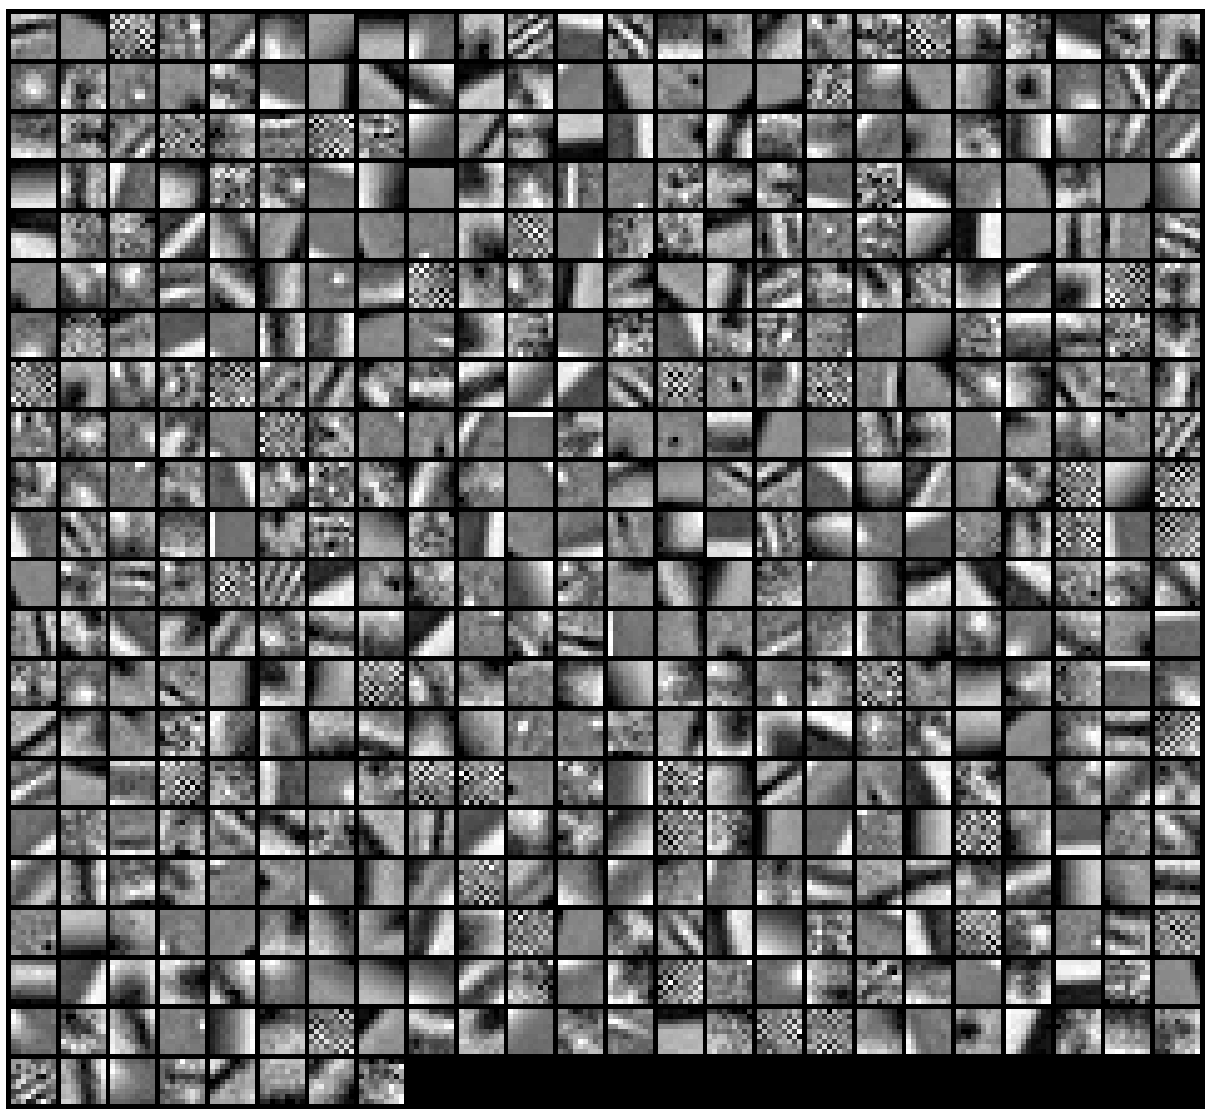
\includegraphics[width=\linewidth,keepaspectratio]{figures/classical/dictpatches.png}
	\caption{512 entry $9 \times 9$ atom HR image patch dictionary trained using 100,000 HR and LR image patch pairs\cite{yang2010}}
	\label{fig:hrpatchdict}
\end{figure}
%
In general dictionary learning minimizes the reconstruction error of the codes across all $J$ example inputs $\bm{Z} \coloneqq \left( \bm{z}_1, \mathellipsis, \bm{z}_J \right)$:
\begin{equation}
	\hat{D} = \underset{D, \bm{A}}{\text{argmin}} \left\| \bm{Z} - D\bm{A} \right\|^2 + \lambda \left\| \bm{A} \right\|_1
\end{equation}
where $\bm{A} \coloneqq \left( \bm{\alpha}_1, \mathellipsis, \bm{\alpha}_J  \right)$.
%
Yang \etal~ "jointly" learn $D_{LR}, D_{HR}$ by making the identifications
\begin{equation*}
	\bm{Z} = \begin{bmatrix}
		\frac{1}{\sqrt{N}}\bY \\ \frac{1}{\sqrt{M}} \bX
	\end{bmatrix} \text{ and }
	D = \begin{bmatrix}
		\frac{1}{\sqrt{N}} D_{HR} \\ \frac{1}{\sqrt{M}} D_{LR}
	\end{bmatrix}
\end{equation*}
where $\bY = \left( \by_1, \mathellipsis, \by_P \right)$ are the example HR patches, $\bX$ similarly the example LR patches, and $N, M$ are the number of HR and LR pixels respectively in each example patch pair $\byi, \bxi$ (in order to normalize the error between $\byi, \bxi$).
\subsubsection{Anchored Neigbhorhood Regression}
Though SC achieves good results for reasonably sized example sets and dictionary sizes it suffers from the inherent computational complexity of solving the optimization problem (see figure~\ref{fig:dictspeedspize}).
\begin{figure}
	\centering
	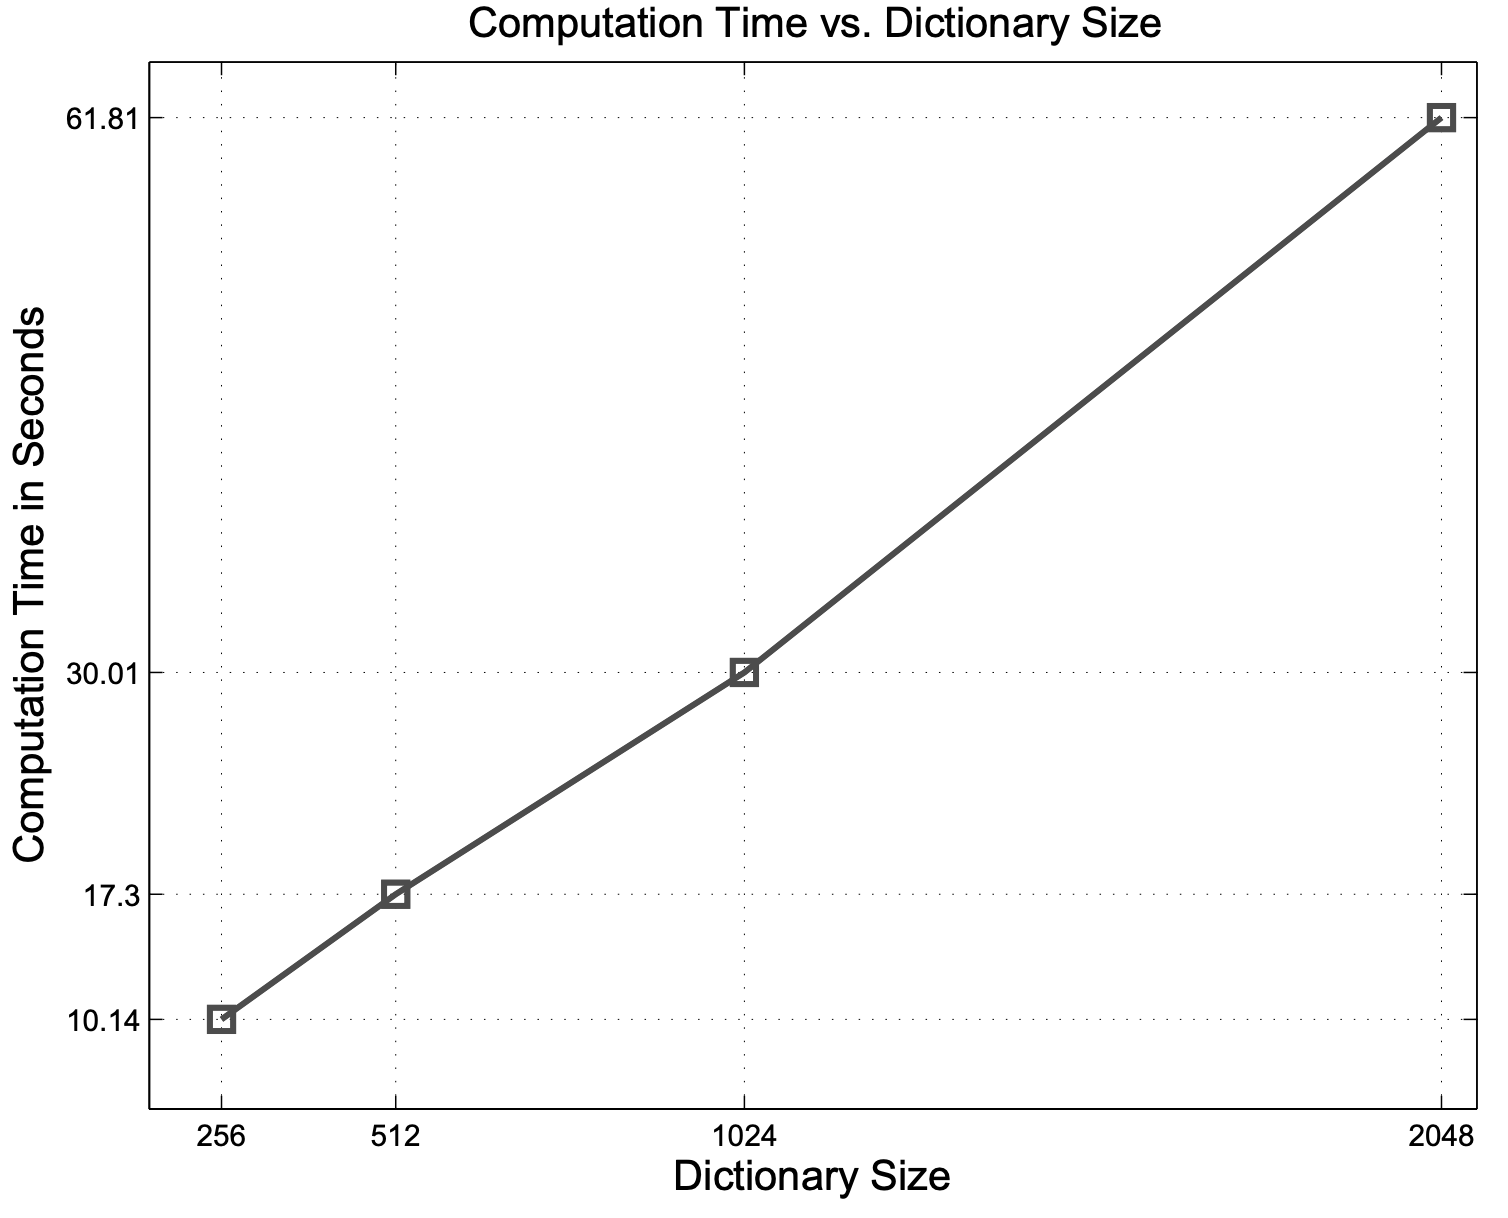
\includegraphics[width=\linewidth,keepaspectratio]{figures/classical/dictsizespeed.png}
	\caption{Dictionary inference time as a function of dictionary size\cite{yang2010}}
	\label{fig:dictspeedspize}
\end{figure}
%
Timofte \etal\cite{Timofte} argues that the chief inefficiency is the $L_1$ norm on the code.
%
By relaxing the $L_1$ norm in eqn.~\eqref{eqn:lagrangerepr} to the $L_2$ norm they recover the Ridge regression form of the problem (see eqn.~\eqref{eqn:closedform}) and get a closed form solution for the code:
\begin{equation}
	\hat{\bm{\alpha}} = \left( D_{LR}^T D_{LR} + \lambda I\right)^{-1}D_{LR}^T \bx
\end{equation}
The code can then be used to compute the HR patch:
\begin{align}
	\by & = D_{HR} \hat{\bm{\alpha}}                                                               \\
	    & = D_{HR} \left( D_{LR}^T D_{LR} + \lambda I\right)^{-1}D_{LR}^T \label{eqn:mappinglr}\bx
\end{align}
Factoring out
\begin{equation}
	P = D_{HR} \left( D_{LR}^T D_{LR} + \lambda I\right)^{-1}D_{LR}^T
\end{equation}
we see that $P$ can be pre-computed, thereby turning inference into simply a matrix multiplication.
%
They then go on to argue, reasoning by analogy with NNE, that the projection should be locally sensitive to input patches, i.e. instead of using the entire dictionary to construct the projection only the atoms nearest to the input LR patch should be used.
%
Thus for every atom in the dictionary, they find its $K' < K$ nearest neighbors, and using only those $K'$ atoms they pre-compute $K$ distinct projection operators $P_k \in \mathbb{R}^{n \times K'}$:
\begin{equation}
	P_k = D_{HR}^k \left( (D_{LR}^k)^T D_{LR}^k + \lambda I\right)^{-1}(D_{LR}^k)^T
	\label{eqn:datadependentmapping}
\end{equation}
where $D_{LR}^k, D_{HR}^k$ are the neighborhood of the LR atom and the neighborhood of its corresponding HR atom.
%
They call these $P_k$ \textit{anchored regressions} because they effectively weight the contributions of LR and HR dictionary atoms.
%
For a new input LR patch $x$ they find the nearest atom in the $D_{LR}$ and recover the HR patch $\by = P_k \bx$.
%
Note that ANR, just as in SC, does not operate on the raw image patches themselves but rather "featurized" image patches: they apply PCA to the first and seconder gradients of the patches and, as in Zeyde \etal\cite{Zeyde2012}, and keep only keep only components explaining 99.9\% of the variance.
%
This reduces the dimensions of their atoms to about 30.
\subsubsection{SR Forests}
Inspired by the anchored regressions of ANR Schulter \etal\cite{Schulter2015} propose a technique called Super-Resolution Forests: their point of departure is a "data-dependent" function $W(\cdot)$ such that
\begin{equation}
	\hat{\by} = W(\bx) \cdot \bx
\end{equation}
This is similar to eqn.~\eqref{eqn:datadependentmapping}.
%
They model $W(\cdot)$ as an $n$-tree regression tree forest.
%
Putting aside for the moment how the trees are trained, each tree $T_t$ independently splits LR patch space into disjoint subspaces by routing patches down the tree (see figure~\ref{fig:firf}).
%
For each tree $t$ each subspace associated with a leaf $l$ is then used to fit a linear basis-regression model defined by
\begin{gather}
	\prescript{l}{t}{W(\bx)} = \sum_{i=1}^I \prescript{l}{t}{\hat{w}_i}\phi_i(\bx) \\
	\prescript{l}{t}{\hat{\bm{w}}} = \underset{\prescript{l}{t}{\bm{w}}}{\text{argmin}} \sum_{j=1}^J \left\| \by_j - \sum_{i=1}^I \prescript{l}{t}{w_i}\phi_i(\bx_j) \right\|^2
	\label{eqn:linearbasisregression}
\end{gather}
where $\prescript{l}{t}{\bm{w}} \coloneqq \left( \prescript{l}{t}{w}_1, \mathellipsis, \prescript{l}{t}{w}_I \right)$ and $\phi_i(\bx_j)$ are basis functions such as the radial basis function
\begin{equation}
	\phi_i(\bx_j) = \exp \left\{ \frac{\left\| \bm{x}_j - \bm{\mu}_i \right\|^2}{\sigma_i} \right\}
\end{equation}
Since the objective in eqn.~\eqref{eqn:linearbasisregression} is linear in $\prescript{l}{t}{w}_i$ the leaf models are fit using the closed form solution to least squares:
\begin{equation}
	\prescript{l}{t}{\hat{\bm{w}}} = \left( \Phi(\bX_t^l)^T \Phi(\bX_t^l) + \lambda I \right)^{-1} \Phi(\bX_t^l)^T \bY_t^l
\end{equation}
where $\bX_t^l$ are only those LR patches that get routed to leaf $l$ in tree $t$, similarly $\bY_t^l$, and $\Phi(\bX_t^l)$ is matrix $\left( \phi_i(\bx_j) \right)$ with $\bx_j$ being one of $\bX_t^l$.
%
\begin{figure}
	\centering
	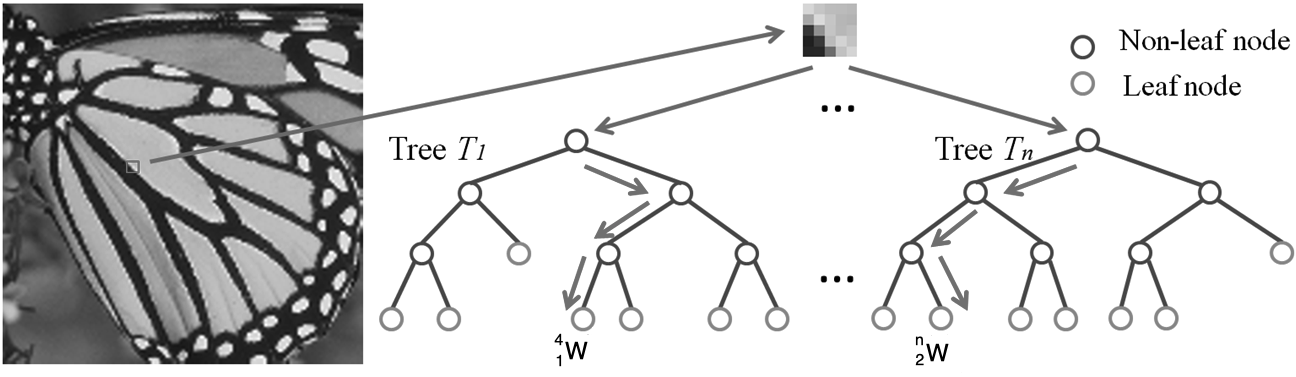
\includegraphics[width=\linewidth,keepaspectratio]{figures/classical/FIRF.png}
	\caption{A set of decision trees. Each decision tree recursively classifies the input LR patch into left or right child node, until a leaf node is reached. By using the linear regression models stored in the each leaf node, the input LR patch can be projected to the HR patch space\cite{Huang}}
	\label{fig:firf}
\end{figure}
%
Finally the inferred HR patch $\by$ is the average of patches $\prescript{l}{t}{W(\bx)}$ inferred by all $n$ trees in the forest:
\begin{equation}
	\hat{\by} = \frac{1}{n} \sum_{t=1}^{n} \prescript{l}{t}{W(\bx)} =  \frac{1}{n} \sum_{t=1}^{n} \sum_{i=1}^I \prescript{l}{t}{\hat{w}_i}\phi_i(\bx)
\end{equation}
where $l = l(t)$ is the leaf that sample $\bx$ is routed to for each tree $t$.
%
Schulter \etal~ train the trees on example LR-HR patch pairs $\bx, \by$ by recursively splitting the data using parameterized splitting functions
\begin{equation}
	\sigma(\bx, i, j, \tau)\coloneqq {
		\begin{cases}
			\text{left}  & \text{if } \text{vec}(\bx)\left[ i \right] - \text{vec}(\bx)\left[ j \right] - \tau < 0 \\
			\text{right} & \text{otherwise}
		\end{cases}
	}
\end{equation}
where $\text{vec}(\bx)\left[ i \right]$ is the $i$th pixel of $\text{vec}(\bx)$ and similarly $\text{vec}(\bx)\left[ j \right]$.
%
The tree is grown as a function of the splitting function, current depth, and current goodness of fit.
%
At each node they select the splitting function parameters $i, j, \tau$ by evaluating all such possible pixel pairs and thresholds according to a "quality measure" whose purpose is to cluster similar LR patches:
\begin{equation}
	Q(\bX, \bY) = \sum_k \left( \left\| \by_k - \hat{\by}_k \right\|^2 + \kappa\left\| \bx_k - \bar{\bx} \right\|^2 \right)
	\label{eqn:qualitymeasure}
\end{equation}
where $\hat{\by}_k$ is the estimate produced by the linear regression fit using data that's arrived at that node.
%
The first term in eqn.~\eqref{eqn:qualitymeasure} measures fitting error and the second term is the clustering regularizer.
%
They decide whether to actually split according to the \textit{error reduction} in performing the split:
\begin{multline*}
	R\left(i, j, \tau, \bX, \bY \right) = \\ Q(\bX, \bY) - \sum_{c\in\left\{L, R\right\}} \frac{|\bX^c|}{|\bX|} Q(\bX^c, \bY^c)
\end{multline*}
where $\bX^L$ are all of the $\bx_k$ such that $\sigma(\bx_k, i, j, \tau) = \text{ left }$ and $\bY^L$ are all the corresponding $\by_k$ (and similarly for $\bX^R, \bY^R$).
%
The best set of parameters $\hat{i}, \hat{j}, \hat{\tau}$ are those that maximize $R\left(i, j, \tau, \bX, \bY \right)$.
%
Then if $R\left(\hat{i}, \hat{j}, \hat{\tau}, \bX, \bY \right)$ is greater than zero (there's an error reduction gained from performing the split) the data is split amongst the left child and right child.
%
Each non-leaf node stores its best set of parameters and each leaf node stores its learned linear regression.

    \section{Deep Learning Algorithms}\label{sec:deep-learning-algorithms}
    \section{Future Research}\label{sec:future-research}
    \section{Conclusion}\label{sec:conclusion}
    \section{Appendix}\label{sec:appendix}
    TODO: work out diffraction circular aperture
    TODO: workout poisson noise
    \section*{Acknowledgments}
    \newpage
    \printbibliography

\end{document}



